%definira klasu dokumenta 
\documentclass[12pt]{report} 

%prostor izmedu naredbi \documentclass i \begin{document} se zove uvod. U njemu se nalaze naredbe koje se odnose na cijeli dokument

%maria

%osnovni LaTex ne može riješiti sve probleme, pa se koriste različiti paketi koji olakšavaju izradu željenog dokumenta
\usepackage[croatian]{babel} 
\usepackage{amssymb}
\usepackage{amsmath}
\usepackage{txfonts}
\usepackage{mathdots}
\usepackage{titlesec}
\usepackage{array}
\usepackage{lastpage}
\usepackage{etoolbox}
\usepackage{longtable, tabu}
\usepackage{color, colortbl}
\usepackage{adjustbox}
\usepackage{geometry}
\usepackage[classicReIm]{kpfonts}
\usepackage{hyperref}
\usepackage{fancyhdr}

\usepackage{float}
\usepackage{setspace}
\restylefloat{table}


\patchcmd{\chapter}{\thispagestyle{plain}}{\thispagestyle{fancy}}{}{} %redefiniranje stila stranice u paketu fancyhdr

%oblik naslova poglavlja
\titleformat{\chapter}{\normalfont\huge\bfseries}{\thechapter.}{20pt}{\Huge}
\titlespacing{\chapter}{0pt}{0pt}{40pt}


\linespread{1.3} %razmak između redaka

\geometry{a4paper, left=1in, top=1in,}  %oblik stranice

\hypersetup{ colorlinks, citecolor=black, filecolor=black, linkcolor=black,	urlcolor=black }   %izgled poveznice


%prored smanjen između redaka u nabrajanjima i popisima
\newenvironment{packed_enum}{
	\begin{enumerate}
		\setlength{\itemsep}{0pt}
		\setlength{\parskip}{0pt}
		\setlength{\parsep}{0pt}
	}{\end{enumerate}}

\newenvironment{packed_item}{
	\begin{itemize}
		\setlength{\itemsep}{0pt}
		\setlength{\parskip}{0pt}
		\setlength{\parsep}{0pt}
	}{\end{itemize}}


%boja za privatni i udaljeni kljuc u tablicama
\definecolor{LightBlue}{rgb}{0.9,0.9,1}
\definecolor{LightGreen}{rgb}{0.9,1,0.9}


%podesavanje zaglavlja i podnožja

\pagestyle{fancy}
\lhead{Programsko inženjerstvo}
\rhead{Zamjena soba}
\lfoot{PiccoloGrupa}
\cfoot{stranica \thepage/\pageref{LastPage}}
\rfoot{\today}
\renewcommand{\headrulewidth}{0.2pt}
\renewcommand{\footrulewidth}{0.2pt}


\begin{document} 
	
	
	
	\begin{titlepage}
		\begin{center}
			\vspace*{\stretch{1.0}} %u kombinaciji s ostalim \vspace naredbama definira razmak između redaka teksta
			\LARGE Programsko inženjerstvo\\
			\large Ak. god. 2020./2021.\\
			
			\vspace*{\stretch{3.0}}
			
			\huge Zamjena soba\\
			\Large Dokumentacija, Rev. \textit{2.}\\
			
			\vspace*{\stretch{12.0}}
			\normalsize
			Grupa: \textit{PiccoloGrupa}\\
			Voditelj: \textit{Maria Katić}\\
			
			
			\vspace*{\stretch{1.0}}
			Datum predaje: \textit{14.1.2021.}\\
	
			\vspace*{\stretch{4.0}}
			
			Nastavnik: \textit{Ivana Cepetić}\\
		
		\end{center}

	
	\end{titlepage}

	
	\tableofcontents

	\chapter{Dnevnik promjena dokumentacije}
		
		\textbf{\textit{Kontinuirano osvježavanje}}\\
				
		
		\begin{longtabu} to \textwidth {|X[2, l]|X[13, l]|X[3, l]|X[3, l]|}
			\hline \multicolumn{1}{|l|}{\textbf{Rev.}}	& \multicolumn{1}{l|}{\textbf{Opis promjene/dodatka}} & \multicolumn{1}{|l|}{\textbf{Autori}} & \multicolumn{1}{l|}{\textbf{Datum}} \\[3pt] \hline
			\endfirsthead
			
			\hline \multicolumn{1}{|l|}{\textbf{Rev.}}	& \multicolumn{1}{l|}{\textbf{Opis promjene/dodatka}} & \multicolumn{1}{|l|}{\textbf{Autori}} & \multicolumn{1}{l|}{\textbf{Datum}} \\[3pt] \hline
			\endhead
			
			\hline 
			\endlastfoot
			
			0.1 & Napravljen predložak.	& Katić & 31.10.2020. 		\\[3pt] \hline 
			0.2 & Dodan Opis projektnog zadatka & Katić & 5.11.2020. \\[3pt] \hline
			0.3	& Arhitektura, dijagram baze podataka, dijagram razreda -  treba doraditi.& Ivezić & 8.11.2020. 	\\[3pt] \hline 
			 
			0.4 & Specifikacija programske potpore, funkcionalni zahtjevi, ostali zahtjevi & Ružić & 10.11.2020. \\[3pt] \hline 
			0.5	& Nadopuna - Arhitektura, dijagram baze podataka, dijagram razreda& Ivezić & 10.11.2020. 	\\[3pt] \hline 
			0.6 & Nadopuna opisa projektnog zadatka & Katić & 11.11.2020. \\[3pt] \hline
			0.7 & Nadopuna specifikacija programske potpore, funkcionalni zahtjevi i ostali zahtjevi & Ružić & 11.11.2020. \\[3pt] \hline 
			0.8 & Dijagrami obrazaca uporabe, sekvencijski dijagrami & Ružić & 12.11.2020. \\[3pt] \hline
			0.9	& Arhitektura, dijagram baze podataka, dijagram razreda -  finalna verzija.& Ivezić & 12.11.2020. 	\\[3pt] \hline 
			{\textbf{1.0}} & Opis projektnog zadatka, specifikacija programske potpore, arhitektura i dizajn sustava (baza podataka, dijagrami razreda) & Ivezić, Katić, Ružić & 13.11.2020. \\[3pt] \hline		
			1.1 & Izmjena baze podataka & Ivezić & 7.1.2021. \\[3pt] \hline
			1.2 & Dodan dijagram komponenti & Katić & 9.1.2021. \\[3pt] \hline
			1.3 & Dodani dijagram stanja i dijagram aktivnosti & Ružić & 9.1.2021. \\[3pt] \hline
			1.4 & Napisan zaključak i korištene tehnologije i alati & Tolj & 9.1.2021. \\[3pt] \hline
			1.5 & Nadopuna Arhitekture & Ivezić & 10.1.2021. \\[3pt] \hline
			1.6 & Dodan dijagram razmještaja & Ružić & 11.1.2021. \\[3pt] \hline
			1.7 & Izmjena UC dijagrama & Ružić & 12.1.2021. \\[3pt] \hline
			1.8 & Napisane upute za puštanje u pogon & Katić & 12.1.2021. \\[3pt] \hline
			1.9 & Dodano ispitivanje komponenti  & Bokan & 13.1.2021. \\[3pt] \hline
			1.9.1 & Dodano ispitivanje sustava  & Katić & 14.1.2021. \\[3pt] \hline
			{\textbf{2.0}} & Konacna verzija &  & 14.1.2021. \\[3pt] \hline
			
			
			
		\end{longtabu}
	
	\chapter{Opis projektnog zadatka}
		

Cilj projektnog zadatka je izrada web aplikacije „Zamjena soba“ koja omogućuje studentima koji žive u studentskim domovima da s lakoćom zamijene sobu s nekim drugim zainteresiranim studentom. Trenutno se ovaj problem rješava usmenim dogovorom studenata ili, još češće, preko društvenih mreža. Nakon toga studenti moraju ići u nadležni Studentski centar da im se odobri zamjena, što također komplicira cijeli postupak. Zamjena soba na ovaj način jako je neorganizirana te zbog nemogućnosti pregleda svih soba koje su dostupne za zamjenu ponekad se dogodi da studenti ne uspiju pronaći idealno rješenje.  \\
		
		Aplikacija „Zamjena soba“ predstavlja soluciju za navedene probleme. Prilikom ulaska u aplikaciju otvara se početna stranica na kojoj se nalaze predani oglasi iz različitih gradova i studentskih domova. Neregistrirani korisnik može gledati oglase, ali preduvjet za korištenje bilo koje druge funkcionalnosti je registracija i/ili prijava u sustav. Neregistriranom korisniku omogućeno je prijavljivanje u sustav s postojećim računom ili izradom novog računa (registracija). Ako se korisnik prijavljuje s postojećim računom potrebno je unijeti korisničko ime i lozinku nakon čega sustav provjera oba podatka i prijavljuje korisnika u sustav. Za kreiranje novog računa potrebno je unijeti:  
		
		\begin{packed_item}
			\item ime
			\item email
			\item JMBAG
			\item korisničko ime
			\item lozinku
		\end{packed_item}
		
		
		Korisnici pri registraciji dobivaju ulogu Studenta, a djelatnicima SC-a su korisnički podaci uneseni direktno u bazu podataka te ne trebaju vršiti registraciju u sustav. \\
		\underbar{Studentu} se prilikom prijave u aplikaciju otvara početna stranica na kojoj se nalaze predani oglasi drugih studenata. Student može otići na stranicu „Predaj oglas“ na kojoj navodi značajke svojeg mjesta u domu: 
		
		\begin{packed_item}
			\item grad
			\item dom
			\item paviljon
			\item kategorija sobe
			\item kat
			\item najbliža menza
		\end{packed_item}

te također navodi značajke mjesta u domu koje želi. Prilikom izrade oglasa za vlastito mjesto mora popuniti sve značajke, a za mjesto koje želi može ostaviti jednu ili više značajki prazno (ako mu ta značajka nije bitna). Student sve svoje oglase može vidjeti na stranici „Moji oglasi“. Tamo se nalaze aktivni i neaktivni oglasi, a aktivni oglasi mogu se uređivati (npr. student može promijeniti značajke domskog mjesta koje želi dobiti). U jednom trenutku samo jedan korisnikov oglas može biti aktivan. Nakon što student unese značajke domskog mjesta koje želi, početna stranica mu se mijenja. Prikazuju se oglasi osoba koje žele onu sobu u domu koju je student oglasio te koje nude sobu koja ima značajke koje je student označio. Također na početnoj stranici su dostupne i sobe koje su u tzv. lancima razmjene (sobe za koje se mogu ostvariti zamjene s tri ili više studenata, a da svatko dobije što želi). Kad se pojave novi oglasi koji odgovaraju navedenim kriterijima, osim što će se pojaviti na početnoj stranici, student će također dobiti obavijest mailom: „Imate nove kandidate za zamjenu sobe u domu!“ s linkom za pregled istih. Sve dostupne oglase student može “lajkati“ , i to po stupnjevima:

	\begin{packed_item}

			\item[] \begin{packed_enum}
				\item sviđa mi se
				\item sviđa mi se jako
				\item to je to
			\end{packed_enum}
			
		\end{packed_item}
		
ili označiti „Ne prikazuj više ovaj oglas“. Kada su obje uključene strane „lajkale“ zamjenu soba, oba studenta bit će obaviještena mailom u kojem će se od njih tražiti da daju konačnu potvrdu zamjene soba. Student će dobiti link u mailu te klikom na taj link otvorit će se stranica za zamjenu na kojoj će student imati mogućnost pregledati zamjenu i prihvatiti željenu sobu. Oba studenta moraju prihvatiti željenu sobu da bi se zamjena dogodila. Nakon što oba studenta prihvate zamjenu, djelatniku SC-a ta zamjena biti će vidljiva i moći će je evidentirati u Studentskom centru.\\

Djelatniku SC-a prilikom prijave u sustav otvaraju se sve zaključane zamjene za studentske domove koji se nalaze u gradu za koji je taj Studentski centar nadležan. Nakon što djelatnik SC-a pogleda neku zamjenu i zabilježi je u sustav SC-a, može je označiti kao obavljenu te se kasnije obavljene zamjene više nigdje ne prikazuju.\\


Rješenje je trenutno izvedeno samo za državne studentske domove, ali moglo bi se prilagoditi za sve studentske domove (privatne i državne) , privatne sobe i stanove u kojima stanuju studenti.\\

Projektni zadatak mogao bi se nadograditi na više načina. Jedan od načina je da student prilikom unosa željenih značajki u domu ima mogućnost navođenja 3 ili 5 tipova soba koje ga zanimaju  tako da značajke mjesta u domu koje ga najviše zanima stavi na prvo mjesto. Na taj način bi student dobio više izbora prilikom traženja sobe za zamjenu. \\

Ovaj projekt uvelike bi olakšao i ubrzao zamjenu soba studentima. Neka sveučilišta u svijetu već su razvila aplikacije koje omogućavaju studentima slične mogućnosti. Jedan primjer aplikacije je aplikacija Sveučilišta u Bostonu koja svojim studentima nudi mogućnost oglašavanja vlastite i pronalaska željene sobe. Za razliku od naše aplikacije koja nudi mogućnost korisnicama da sami pregledavaju oglase i označavaju one koje im se sviđaju, aplikacija Sveučilišta u Bostonu nema tu mogućnost. Sustav sam pronalazi moguće zamjene i šalje ih na mail zainteresiranim studentima koji nakon toga trebaju provesti potvrdu. \\

Slika 2.1 prikazuje stranicu aplikacije za zamjenu soba Sveučilišta u Bostonu na kojoj je prikazana ponuda za zamjenu soba koju je student dužan potvrditi ukoliko želi da se zamjena ostvari. Ova funkcionalnost implementirana je i u našoj aplikaciji.

%unos slike
		\begin{figure}[H]
			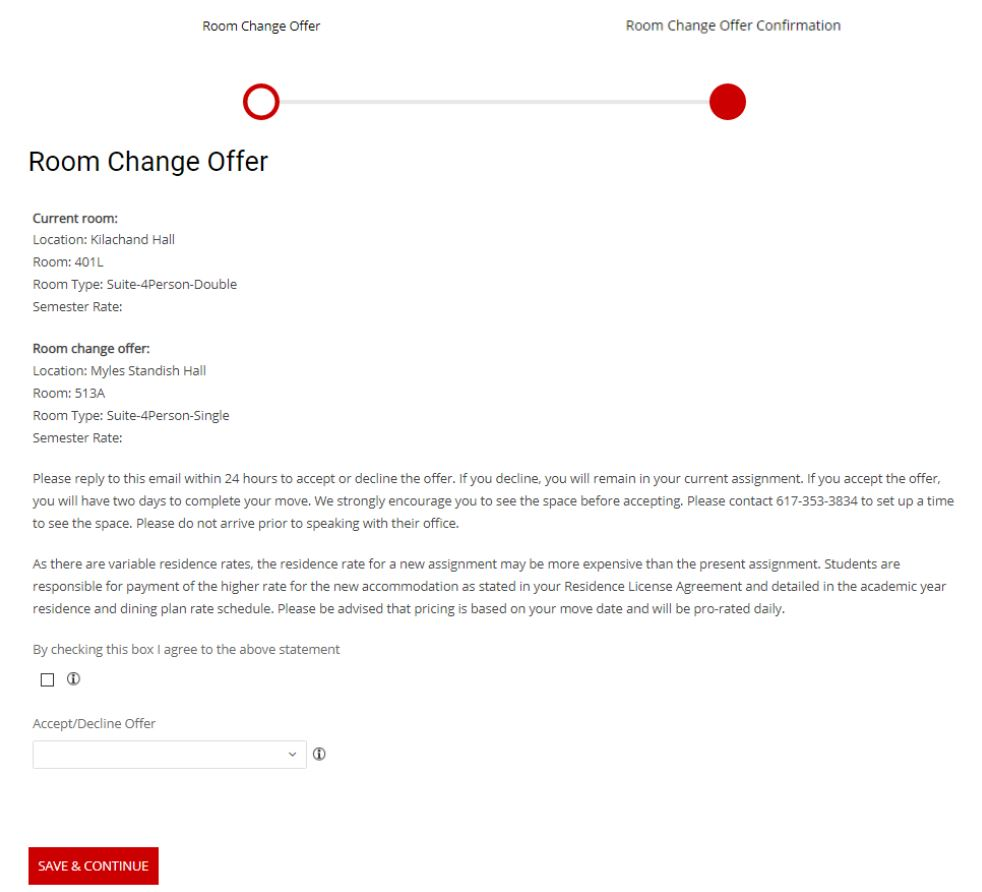
\includegraphics[scale=0.4]{slike/pic1.JPG} %veličina slike u odnosu na originalnu datoteku i pozicija slike
			\centering
			\caption{Aplikacija za zamjenu soba Sveučilišta u Bostonu}
			\label{fig:promjene1}
		\end{figure}

	
	\chapter{Specifikacija programske potpore}

\section{Funkcionalni zahtjevi}

\noindent \textbf{Dionici:}

\begin{packed_enum}
	
	\item Studenti
	\item Djelatnici studentskog centra			
	\item Razvojni tim
	
\end{packed_enum}

\noindent \textbf{Aktori i njihovi funkcionalni zahtjevi:}


\begin{packed_enum}
	\item  \underbar{Neregistrirani klijent (inicijator) može:}
	
	\begin{packed_enum}
		
		\item vidjeti predane oglase
		\item registrirati se u sustav, stvoriti novi korisnički račun i kasnije se prijaviti u sustav
		
	\end{packed_enum}
	
	\item  \underbar{Registrirani korisnik (student) (inicijator) može:}
	
	\begin{packed_enum}
		
		\item prijaviti se u sustav i odjaviti se iz sustava
		\item predati oglas za zamjenu sobe sa značajkama njegove sobe i željama sobe za zamjenu
		\item pregledati i uređivati vlastiti profil 
		\item vidjeti svoje aktivne i neaktivne oglase
		\item uređivati svoje aktivne oglase (promjeniti detalje oglasa ili ga učiniti neaktivnim)
		\item vidjeti oglase drugih korisinka te ih „lajkati“ ili označiti da se više ne prikazuje
		\item pregledati oglase koji odgovaraju njegovim kriterijima
		\item pregledati zaprimljene ponude za zamjenu
		\item potvrditi zamjenu soba
		
	\end{packed_enum}
		
	\item  \underbar{Djelatnik studentskog centra (sudionik) može:}
	
	\begin{packed_enum}
		
		\item vidjeti potvrđene (zaključane) zamjene između studenata
		\item označiti potvrđene zamjene koje je unio u sustav studentskog centra kao obavljene
		
	\end{packed_enum}
	
	\item  \underbar{Baza podataka (sudionik) može:}
	
	\begin{packed_enum}
		
		\item pohranjuje sve podatke o korisnicima
		\item pohranjuje sve podatke o predanim oglasima
		\item pohranjuje sve podatke o zamjenama
		
	\end{packed_enum}
\end{packed_enum}

\eject 



\subsection{Obrasci uporabe}


\subsubsection{Opis obrazaca uporabe}


\noindent \underbar{\textbf{UC1 - Pregledaj oglase}}
\begin{packed_item}
	
	\item \textbf{Glavni sudionik: } neregistrirani klijent, registrirani korisnik
	\item  \textbf{Cilj:} pregled ponude predanih oglasa
	\item  \textbf{Sudionici:} baza podataka
	\item  \textbf{Preduvjet:} -
	\item  \textbf{Opis osnovnog tijeka:}
	
	\item[] \begin{packed_enum}
		
		\item neregistrirani klijent/registrirani korisnik otvara aplikaciju
		\item sustav prikazuje predane oglase
		\item  neregistrirani klijent/registrirani korisnik listanjem aplikacije(„scrollanjem“) prema dolje može vidjeti još oglasa
		
	\end{packed_enum}
	
\end{packed_item}


\noindent \underbar{\textbf{UC2 - Registriraj korisnika}}
\begin{packed_item}
	
	\item \textbf{Glavni sudionik: } neregistrirani klijent
	\item  \textbf{Cilj:} stvaranje korisničkog računa koji omogućuje prijavu u sustav i predaju oglasa
	\item  \textbf{Sudionici:} baza podataka
	\item  \textbf{Preduvjet:} ispravna e-mail adresa i važeći JMBAG
	\item  \textbf{Opis osnovnog tijeka:}
	
	\item[] \begin{packed_enum}
		
		\item neregistrirani klijent u izborniku koji se nalazi u gornjem desnom kutu aplikacije odabire opciju za registraciju („Registriraj se“)
		\item sustav neregistriranog klijenta vodi na stranicu za registraciju na kojoj traži njegove korisničke podatke
		\item klijent unosi korisničko ime, e-mail adresu, JMBAG, ime i prezime te lozinku
		\item klijent odabire opciju za registraciju („Registriraj se“) koja se nalazi ispod unešenih podataka
		\item sustav prikazuje prikladnu poruku o uspješnoj registraciji 
		
	\end{packed_enum}
	
	\item  \textbf{Opis mogućih odstupanja:}
	
	\item[] \begin{packed_item}
		
		\item[3.a] odabrano korisničko ime je zauzeto ili je već postoji račun sa istom e-mail adresom
		\item[] \begin{packed_enum}
			
			\item sustav prikazuje prikladnu poruku  „Korisničko ime je zauzeto“ ili „Već postoji račun sa ovom e-mail adresom“
			
		\end{packed_enum}
	
		\item[3.b] korisnik nije unio sve potrebne podatke za registraciju (korisničko ime, e-mail adresu, JMBAG, ime i prezime ili lozinku)
		\item[] \begin{packed_enum}
			
			\item sustav prikazuje prikladnu poruku o potrebi za ispunjavanjem svih polja o korisničkim podacima
			
		\end{packed_enum}
		
	\end{packed_item}
\end{packed_item}


\noindent \underbar{\textbf{UC3 - Prijavi korisnika}}
\begin{packed_item}
	
	\item \textbf{Glavni sudionik: } registrirani korisnik (student ili djelatnik studentskog centra)
	\item  \textbf{Cilj:} pristupanje korisničkom sučelju, predaja oglasa
	\item  \textbf{Sudionici:} baza podataka
	\item  \textbf{Preduvjet:} registracija
	\item  \textbf{Opis osnovnog tijeka:}
	
	\item[] \begin{packed_enum}
		
		\item registrirani korisnik u izborniku u gornjem desnom kutu aplikacije odabire opciju za prijavu („Prijavi se“)
		\item sustav korisnika vodi na stranicu za prijavu na kojoj traži korisničko ime i lozinku te mu ispod podataka koje traži nudi gumb za prijavu („Prijavi se“)
		\item korisnik upisuje tražene podatke te odabire opciju za prijavu („Prijavi se“) 
		\item sustav obavještava korisnika o uspješnoj prijavi te mu dozvoljava pristup korisničkom sučelju
	
		
	\end{packed_enum}
	
	\item  \textbf{Opis mogućih odstupanja:}
	
	\item[] \begin{packed_item}
		
		\item[4.a] neispravan unos korisničkog imena ili  lozinke
		\item[] \begin{packed_enum}
			
			\item sustav obavještava korisnika o neuspjeloj prijavi te mu nudi ponovni pokušaj
			
		\end{packed_enum}

	\end{packed_item}
\end{packed_item}



	\noindent \underbar{\textbf{UC4 - Odjavi korisnika}}
	\begin{packed_item}
		
		\item \textbf{Glavni sudionik: } registrirani korisnik (student ili djelatnik studentskog centra)
		\item  \textbf{Cilj:} odjava iz korisničkog sučelja
		\item  \textbf{Sudionici:} baza podataka
		\item  \textbf{Preduvjet:} registracija, prijava
		\item  \textbf{Opis osnovnog tijeka:}
		
		\item[] \begin{packed_enum}
			
			\item registrirani korisnik u izborniku u gornjem desnom kutu aplikacije odabire opciju za odjavljivanje („Odjava“)	
			\item sustav odjavljuje korisnika te ga vodi na početnu stranicu gdje može vidjeti oglase svih korisnika, a u gornjem desnom kutu aplikacije, u izborniku ima opcije  „Početna“, „Prijavi se“ i „Registriraj se“ 
		\end{packed_enum}
	
	\end{packed_item}

\noindent \underbar{\textbf{UC5 - Predaj oglas}}
\begin{packed_item}
	
	\item \textbf{Glavni sudionik: } registrirani korisnik
	\item  \textbf{Cilj:} predaja vlastitog oglasa u sustav
	\item  \textbf{Sudionici:} baza podataka
	\item  \textbf{Preduvjet:} registracija, prijava
	\item  \textbf{Opis osnovnog tijeka:}
	
	\item[] \begin{packed_enum}
		
		\item registrirani korisnik odabire opciju za pregled vlastith oglasa („Moji oglasi“) koja se nalazi u izborniku u gornjem desnom kutu aplikacije 
		\item sustav vodi korisnika na stranicu na kojoj se nalaze svi neaktivni oglasi korisnika te mu na gornjem dijelu ekrana nudi opciju za stvaranje novog oglasa
		\item korisnik odabire opciju za stvaranje novog oglasa
		\item sustav vodi korisnika na stranicu za predaju novog oglasa, na kojoj od njega traži značajke (grad, dom, paviljon, kategorija sobe, kat, najbliža menza) njegove sobe u domu (ispunjavanje svih podataka o sobi koju korisnik nudi je obavezno)
		\item korisnik ispunjuje tražene podatke te odabire opciju „Predaj oglas“ koja se nalazi ispod kućica za upis traženih podataka
		\item sustav korisniku ispisuje poruku o uspješnoj predaji oglasa te ga vraća na stranicu „Moji oglasi“
		\item ukoliko je korisnik imao aktivan oglas prilikom predaje novog oglasa, on predajom novog oglasa automatski postaje neaktivan jer jedan korisnik može imati najviše jedan aktivan oglas istovremeno
		\item korisnik zatim vidi svoj novi aktivan oglas i sve neaktivne oglase
		
	\end{packed_enum}


\item  \textbf{Opis mogućih odstupanja:}

\item[] \begin{packed_item}
	
	\item[6.a] korisnik nije unio sve obavezne podatke (grad, dom, paviljon, kategorija sobe, kat, najbliža menza) o sobi koju nudi
	\item[] \begin{packed_enum}
		
		\item korisnik ne može predati oglas dok ne ispuni sve obavezne podatke
		\item sustav ispisuje odgovarajuću obavijest
		
	\end{packed_enum}
	
\end{packed_item}
	
\end{packed_item}



\noindent \underbar{\textbf{UC6 - Pregledaj vlastite oglase}}
\begin{packed_item}
	
	\item \textbf{Glavni sudionik: } registrirani korisnik
	\item  \textbf{Cilj:} pregled vlastitih predanih oglasa
	\item  \textbf{Sudionici:} baza podataka
	\item  \textbf{Preduvjet:} registracija, prijava
	\item  \textbf{Opis osnovnog tijeka:}
	
	\item[] \begin{packed_enum}
		
		\item registrirani korisnik odabire opciju za pregled vlastith oglasa koja se nalazi u izborniku u gornjem desnom kutu aplikacije („Moji oglasi“)
		\item sustav vodi korisnika na stranicu na kojoj se nalaze svi neaktivni oglasi korisnika, aktivan oglas (ako takav postoji) te opcija za stvaranje novog oglasa
		\item ukoliko korisnik ima više oglasa može ih pogledati listanjem aplikacije („scrollanjem“) prema dolje
		\item korisnik se može vratiti na početnu stranicu klikom na „Početna“ u izborniku u gornjem desnom kutu aplikacije
		
		
	\end{packed_enum}
	
	\item  \textbf{Opis mogućih odstupanja:}
	
	\item[] \begin{packed_item}
		
		\item[2.a] nepostojanje oglasa
		\item[] \begin{packed_enum}
			
			\item sustav ispisuje prikladnu poruku o nepostojanju oglasa
			\item sustav nudi korisniku da stvori oglas
			
		\end{packed_enum}
		
	\end{packed_item}
	
\end{packed_item}


\noindent \underbar{\textbf{UC7 - Uredi oglas}}
\begin{packed_item}
	
	\item \textbf{Glavni sudionik: } registrirani korisnik
	\item  \textbf{Cilj:} promjena detalja oglasa
	\item  \textbf{Sudionici:} baza podataka
	\item  \textbf{Preduvjet:} registracija, prijava, postojanje oglasa
	\item  \textbf{Opis osnovnog tijeka:}
	
	\item[] \begin{packed_enum}
		
		\item registrirani korisnik odabire opciju za pregled vlastith oglasa koja se nalazi u izborniku u gornjem desnom kutu aplikacije („Moji oglasi“)
		\item sustav vodi korisnika na stranicu na kojoj se nalazi aktivan oglas ukoliko postoji i svi neaktivni oglasi korisnika
		\item korisnik odabire opciju za uređivanje oglasa u donjem desnom kutu oglasa kojeg želi urediti („uredi“)
		\item sustav korisnika vodi na stranicu „Uredi oglas“ na kojoj korisnik može promijeniti bilo koji detalj vezan za oglas
		\item korisnik po želji mijenja podatke o oglasu
		\item sustav na dnu stranice za uređivanje oglasa nudi korisniku opcije „Spremi promjene“
		\item korisnik odabirom opcije „Spremi promjene“ mijenja detalje oglasa
		\item nakon odabira opcije „Spremi promjene“ ili odabira izlaska iz stranice za uređivanje oglasa (X u gornjem desnom kutu), sustav vraća korisnika na stranicu „Moji oglasi“ gdje se sada nalazi izmjenjen oglas(ukoliko je korisnik odabrao opciju „Spremi promjene“), ili oglas koji je isti kao i prije (ukoliko je korisnik odabrao izaći bez promjena)
		\item korisnik se može vratiti na početnu stranicu klikom na „Početna“ u izborniku u gornjem desnom kutu aplikacije
		
	\end{packed_enum}
	
\end{packed_item}


	

\noindent \underbar{\textbf{UC8 - Uredi profil}}
\begin{packed_item}
	
	\item \textbf{Glavni sudionik: } registrirani korisnik (student ili djelatnik studentskog centra)
	\item  \textbf{Cilj:}  promjena detalja profila
	\item  \textbf{Sudionici:} baza podataka
	\item  \textbf{Preduvjet:} registracija, prijava
	\item  \textbf{Opis osnovnog tijeka:}
	
	\item[] \begin{packed_enum}
		
		\item korisnik odabire opciju „Uredi profil“ u izborniku u gornjem desnom kutu aplikacije 
		\item sustav prikazuje korisniku njegove korisničke podatke (korisničko ime, ime i prezime, JMBAG, e-mail adresu)
		\item korisnik odabire opciju „uredi“ koja se nalazi ispod svih podataka
		\item sustav omogućuje korisniku promjenu bilo kojeg od podataka ili promjenu lozinke 
		\item korisnik mijenja željene podatke
		\item sustav korisniku nudi opcije „Ažuriraj podatke“ i „Ažuriraj lozinku“
		\item korisnik odabire jednu od ponuđenih opcija
		\item sustav ponovno prikazuje korisniku njegove korisničke podatke koji su izmjenjeni ili isti(ukoliko je mijenjao lozinku), ovisno o korisnikovom ranijem odabiru
		\item korisnik se može vratiti na početnu stranicu klikom na „Početna“ u izborniku u gornjem desnom kutu aplikacije
			
	\end{packed_enum}
	
\end{packed_item}



\noindent \underbar{\textbf{UC9 - Reagiraj na oglas}}
\begin{packed_item}
	
	\item \textbf{Glavni sudionik: } registrirani korisnik
	\item  \textbf{Cilj:}  izraziti želju za zamjenom sobe s korisnikom koji je dao oglas ili spriječiti ponovno pojavljivanje određenog oglasa
	\item  \textbf{Sudionici:} baza podataka
	\item  \textbf{Preduvjet:} registracija, prijava, postojanje aktivnog oglasa
	\item  \textbf{Opis osnovnog tijeka:}
	
	\item[] \begin{packed_enum}
		
		\item registrirani korisnik želi reagirati na određeni oglas
		\item korisnik odabire jednu od opcija za reagiranje na oglas koje su prikazane simbolom 1, 2 ili 3 srca, tj. kantom za smeće
		\item opcije koje su prikazane simbolima srca označuju stupanj sviđanja (1-malo, 3-jako), dok opcija koja je prikazana simbolom kante za smeće označuje da korisnik ne želi da mu se taj oglas više prikazuje
		\item ako je oglas „lajkan“ sustav šalje e-mail korisniku čiji je oglas „lajkan“ koji sadrži poruku „Imate nove kandidate za zamjenu sobe u domu!“ te link na stranicu „Dobiveni lajkovi“ koja se nalazi u izborniku u gornjem desnom kutu aplikacije gdje korisnik može vidjeti aktivne oglase svih korisnika koji su „lajkali“ njegov aktivan oglas
			
	\end{packed_enum}

\end{packed_item}

	

\noindent \underbar{\textbf{UC10 - Pregledaj oglase koji odgovaraju kriterijima}}
\begin{packed_item}
	
	\item \textbf{Glavni sudionik: } registrirani korisnik
	\item  \textbf{Cilj:}  pronalazak sobe za zamjenu
	\item  \textbf{Sudionici:} baza podataka
	\item  \textbf{Preduvjet:} registracija, prijava, postojanje aktivnog oglasa
	\item  \textbf{Opis osnovnog tijeka:}
	
	\item[] \begin{packed_enum}
		
		\item korisnik na početnoj stranici odabire opciju „Filtracija oglasa“
		\item korisnik unosi podatke o željenoj sobi te odabire opciju „Pretraži“
		\item korisnik također može odabrati i opcije „Spremi filter“ koja mu omogućuje spremanje unešenog filtera i „Prikaži spremljene filtere“ koja mu omogućuje prikaz do sada spremljenih oglasa
		\item korisnik može reagirati na bilo koji od oglasa koji su dobiveni filtriranjem
		
	\end{packed_enum}

\end{packed_item}



\noindent \underbar{\textbf{UC11 - Pregledaj zaprimljene ponude za zamjenu}}
\begin{packed_item}
	
	\item \textbf{Glavni sudionik: } registrirani korisnik
	\item  \textbf{Cilj:}  pregled oglasa onih korisnika koji žele zamjeniti sobu sa korisnikom
	\item  \textbf{Sudionici:} baza podataka
	\item  \textbf{Preduvjet:} registracija, prijava, postojanje aktivnog oglasa
	\item  \textbf{Opis osnovnog tijeka:}
	
	\item[] \begin{packed_enum}
		
		\item korisnik odabire opciju „Dobiveni lajkovi" koja se nalazi u izborniku u gornjem desnom kutu aplikacije
		\item sustav vodi korisnika na stranicu na kojoj mu prikazuje oglase studenata koji su „lajkali“ njegov oglas 
		\item korisnik pregledava zaprimljene ponude za zamjenu te po želji reagira na njih
		
	\end{packed_enum}
	
	\item  \textbf{Opis mogućih odstupanja:}
	
	\item[] \begin{packed_item}
		
		\item[2.a] nema novih kandidata za zamjenu
		\item[] \begin{packed_enum}
			
			\item sustav ispisuje prikladnu poruku
			
		\end{packed_enum}
	\end{packed_item}
\end{packed_item}



\noindent \underbar{\textbf{UC12 - Potvrdi zamjenu}}
\begin{packed_item}
	
	\item \textbf{Glavni sudionik: } registrirani korisnik
	\item  \textbf{Cilj:}  konačni odabir zamjene soba
	\item  \textbf{Sudionici:} baza podataka
	\item  \textbf{Preduvjet:} registracija, prijava, postojanje aktivnog oglasa, međusobno „lajkanje“ oglasa dvoje korisnika
	\item  \textbf{Opis osnovnog tijeka:}
	
	\item[] \begin{packed_enum}
		
		\item korisnik odlazi na stranicu „Moguće zamjene“ koja se nalazi u izborniku u gornjem desnom kutu aplikacije
		\item korisnik dolazi na stranicu na kojoj se prikazuje oglas ponuđene sobe za potvrdu zamjene (oglas može ponovno pogledati) te se ispod njega nalaze opcije „Potvrdi zamjenu“ i „Odbij zamjenu“
		\item korisnik potvrđuje zamjenu odabirom opcije „Potvrdi zamjenu“ ili ju odbija odabirom opcije „Odbij zamjenu“
		\item ukoliko svi korisnici uključeni u zamjenu potvrde zamjenu, djelatnik studentskog centra dobiva podatke o zamjeni, a ukoliko barem jedan od korisnika uključenih u zamjenu odbije zamjenu, svi uključeni u zamjenu dobivaju e-mail o neuspjelom ostvarenju zamjene
		
	\end{packed_enum}
	
	\item  \textbf{Opis mogućih odstupanja:}
	
	\item[] \begin{packed_item}
		
		\item[3.a] svi korisnici uključeni u zamjenu nisu potvrdili niti odbili zamjenu
		\item[] \begin{packed_enum}
			
			\item sustav nakon 7 dana briše ponudu za potvrdu ili odbijanje zamjene te se ona automatski smatra neostvarenom
			\item sustav šalje svim korisnicima uključenim u zamjenu e-mail o neuspjelom ostvarenju zamjene 
			
		\end{packed_enum}

		\item[3.b] jedan ili više korisnika uključenih u zamjenu je učinio svoj oglas neaktivnim, a drugi korisnik (korisnici) su potvrdili zamjenu
		\item[] \begin{packed_enum}
			
			\item sustav šalje svim korisnicima uključenim u zamjenu e-mail o neuspjelom ostvarenju zamjene
			
		\end{packed_enum}
		
		
	\end{packed_item}
\end{packed_item}

\noindent \underbar{\textbf{UC13 - Pregledaj zaključane zamjene i označi one obrađene}}
\begin{packed_item}
	
	\item \textbf{Glavni sudionik: } radnik studentskog centra
	\item  \textbf{Cilj:}  potvrda zamjene soba u sustavu studentskog centra i označavanje obrađenih zamjena
	\item  \textbf{Sudionici:} baza podataka
	\item  \textbf{Preduvjet:}  prijava, postojanje zaključanih zamjena
	\item  \textbf{Opis osnovnog tijeka:}
	
	\item[] \begin{packed_enum}
		
		\item radnik studentskog centra odabire opciju „Prikaži zaključane zamjene“ koja se nalazi u izborniku u gornjem desnom kutu aplikacije
		\item sustav radniku studentskog centra  prikazuje jednu po jednu zaključanu zamjenu te ispod svake zamjene nudi opciju „Zamjena obrađena“
		\item radnik studentskog centra unosi zaključanu zamjenu u sustav studentskog cetra te odabire opciju „Zamjena obrađena“ kako bi označio obrađene zamjene
		\item sustav unosi podatke o obrađenoj zamjeni u bazu podataka, korisnicima kojma su sobe uspješno zamjenjene šalje prikladan e-mail te obrađenu zamjenu više ne prikazuje radniku studentskog centra
		\item sustav radniku studentskog centra prikazuje iduću zaključanu zamjenu
		
	\end{packed_enum}
	
\end{packed_item}

\eject

\subsubsection{Dijagram obrazaca uporabe}

\begin{figure}[H]
	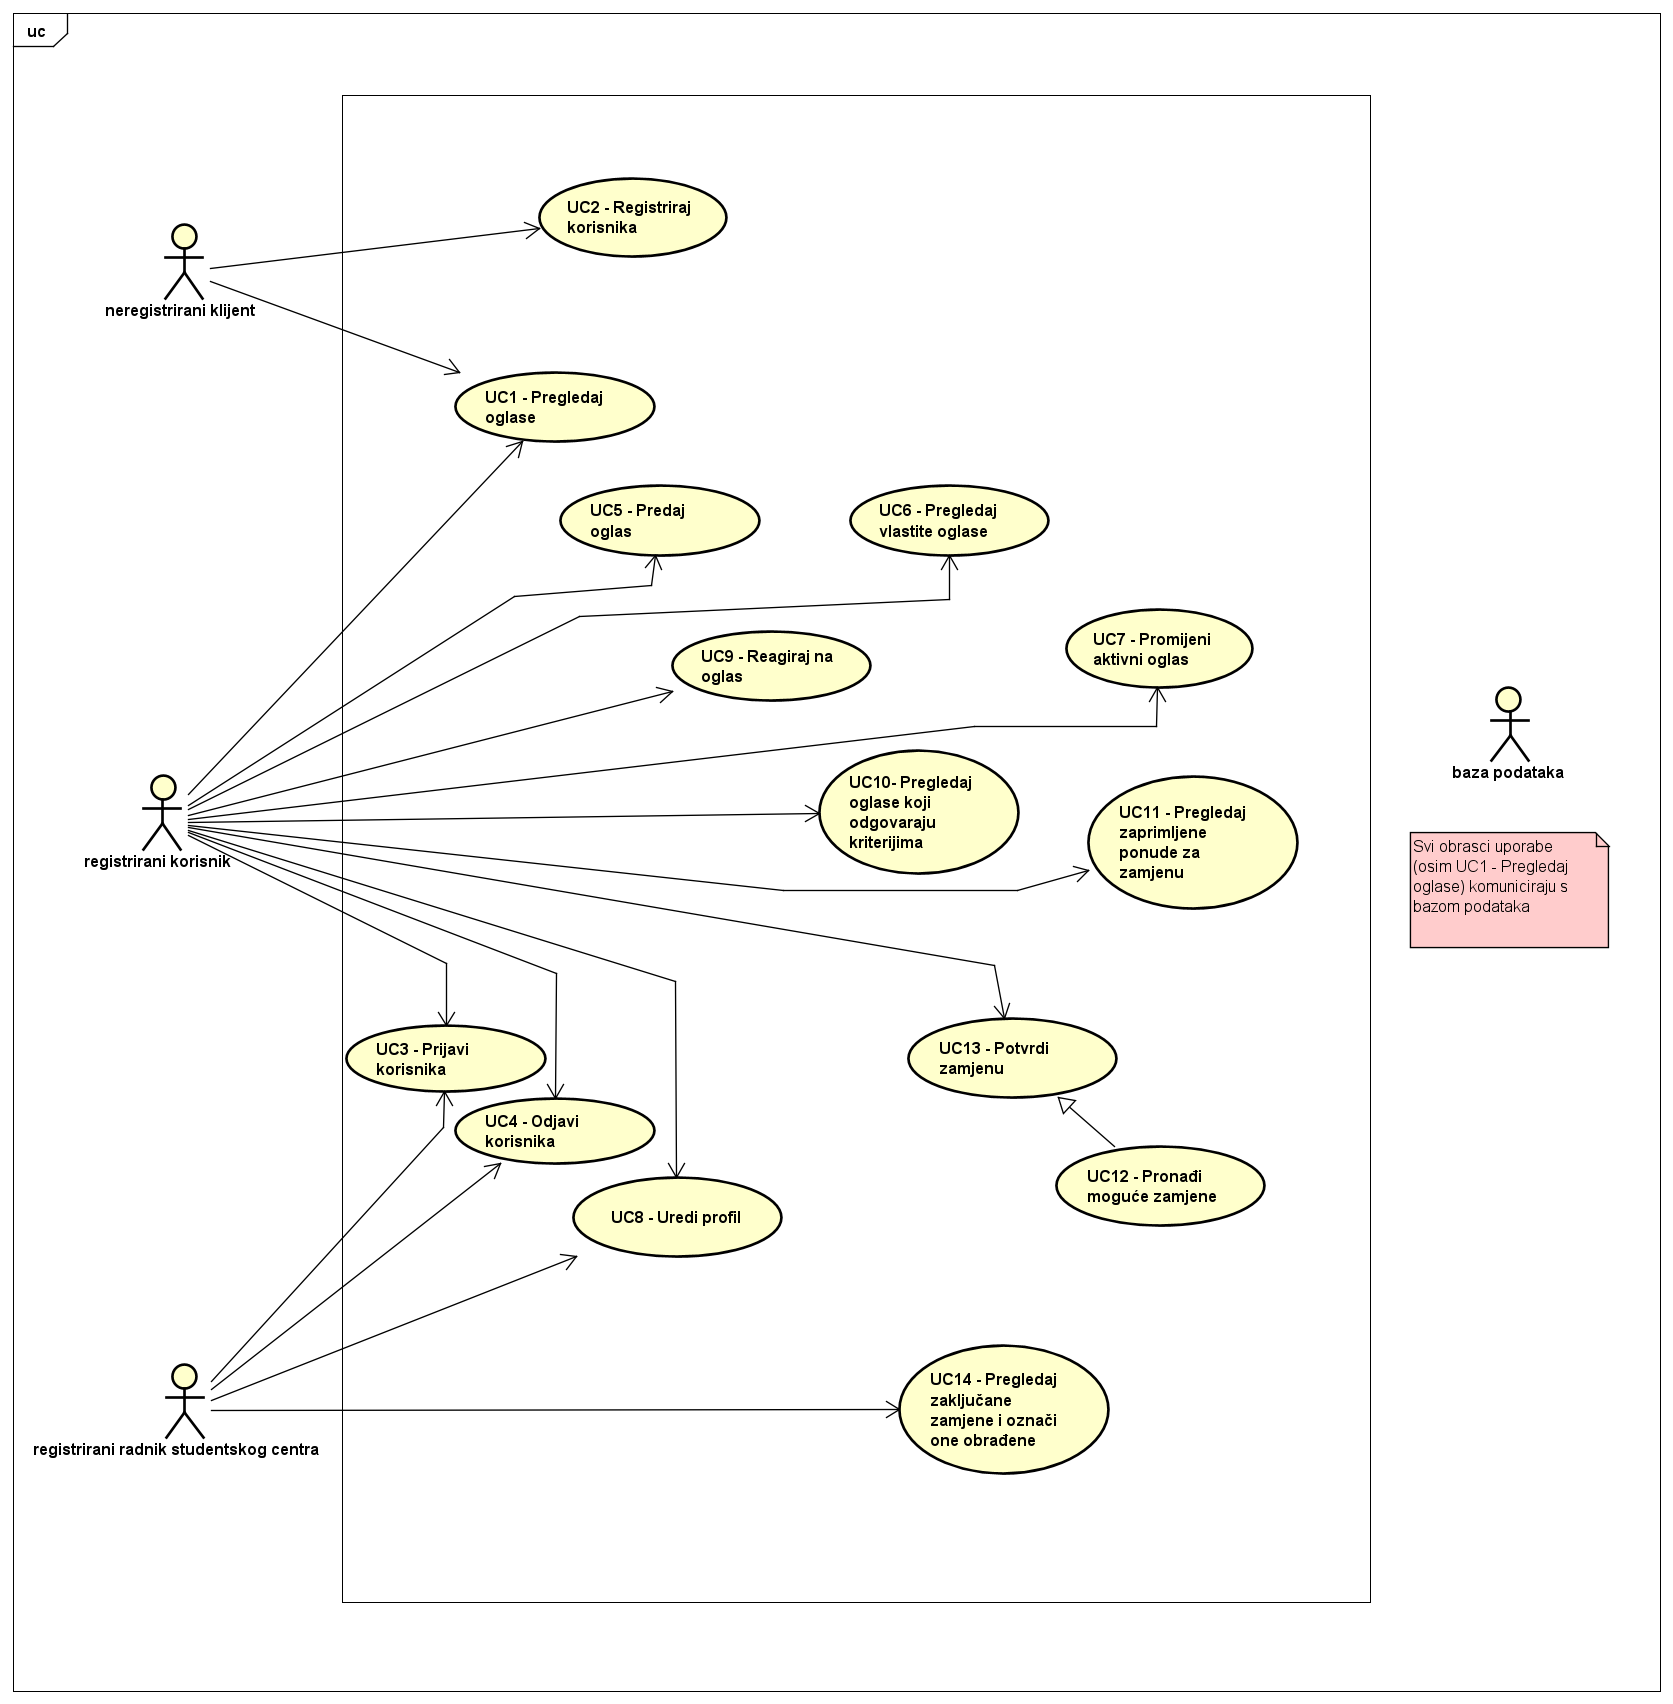
\includegraphics[width=.9\linewidth]{slike/UC_Diagram.PNG} %veličina u odnosu na širinu linije
	\centering
	\caption{Dijagram obrazaca uporabe}
	\label{fig:UC_Diagram} %label mora biti drugaciji za svaku sliku
\end{figure}

\eject	

\subsection{Sekvencijski dijagrami}
	
		\textbf{UC5 - Predaj oglas}
		\textit\\
		Registrirani korisnik šalje zahtjev za pregled vlastitih oglasa. Poslužitelj dohvaća korisnikove oglase iz baze podataka te ih prikazuje korisniku. Korisnik šalje zahtjev za stvaranje novog oglasa a poslužitelj mu vraća stranicu za stvaranje novog oglasa. Korisnik ispunjava novi oglas te šalje zahtjev za spremanje oglasa. Poslužitelj sprema oglas u bazu podataka i korisniku ispisuje poruku „Oglas uspješno predan“.

	
	\begin{figure}[H]
		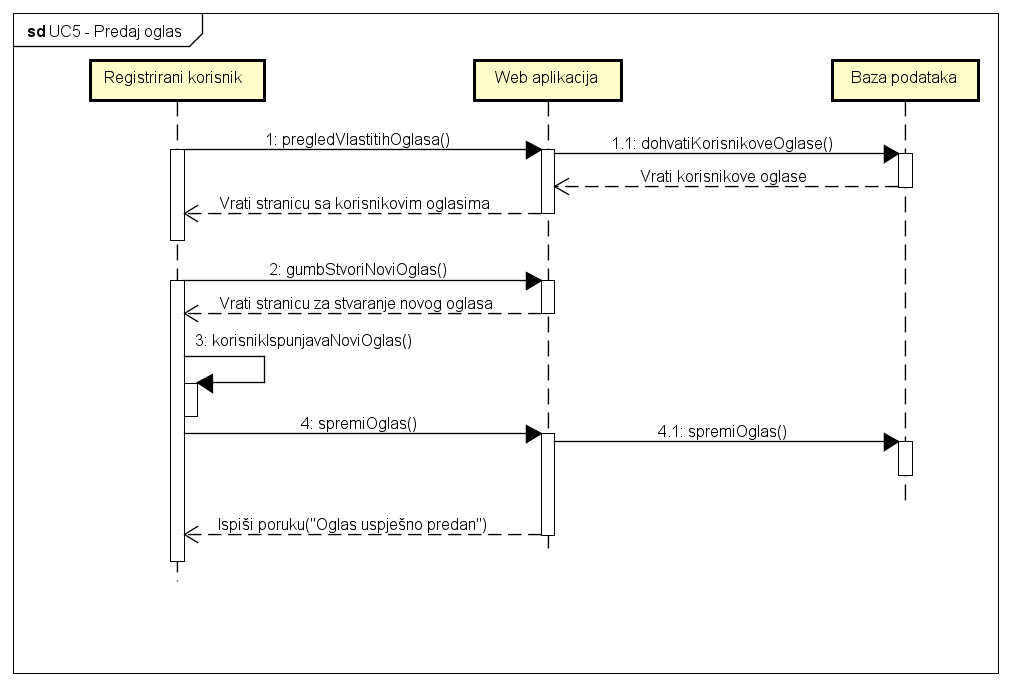
\includegraphics[width=.9\linewidth]{slike/UC5_sekvencijski_dijagram.PNG} %veličina u odnosu na širinu linije
		\centering
		\caption{Sekvencijski dijagram za UC5}
		\label{fig:sekvdij} %label mora biti drugaciji za svaku sliku
	\end{figure}

\eject
	
	\textbf{UC11 - Pregledaj zaprimljene ponude za zamjenu}
		\textit\\
		Registrirani korisnik šalje zahtjev za prikaz kandidata za zamjenu kako bi vidio oglase korisnika koji su  „lajkali“ njegov oglas i koji bi se htjeli zamjeniti za sobe sa njime. Poslužitelj dohvaća kandidate za zamjenu iz baze podataka i prikazuje ih korisniku. Ukoliko ne postoje kandidati za zamjenu poslužitelj prikazuje poruku  „Ne postoje kandidati za zamjenu“.  
		
	
	\begin{figure}[H]
		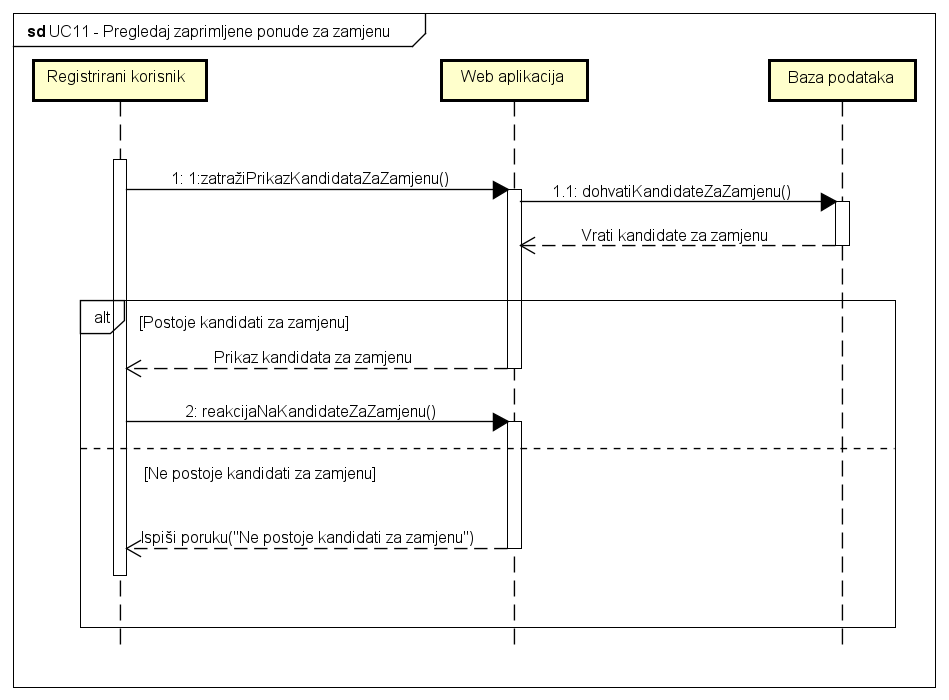
\includegraphics[width=.9\linewidth]{slike/UC11_sekvencijski_dijagram.PNG} %veličina u odnosu na širinu linije
		\centering
		\caption{Sekvencijski dijagram za UC11}
		\label{fig:sekvdij1} %label mora biti drugaciji za svaku sliku
	\end{figure}

\eject
	
		\textbf{UC13 - Potvrdi zamjenu}
		\textit\\
		Poslužitelj šalje korisniku e-mail za potvrdu zamjene. Registrirani korisnik klikne na link (odabere ga) te dolazi na web aplikaciju koja ga preusmjerava na stranicu za potvrdu. Korisnik potvrđuje ili odbija zamjenu, poslužitelj sprema promjenu u bazu podataka, te ako svi korisinici uključeni u zamjenu potvrde zamjenu poslužitelj ispisuje poruku „Zamjena potvrđena“, a ako jedan ili više korisnika uključenih u zamjenu odbiju zamjenu poslužitelj svim korisnicima uključenim u zamjenu ispisuje poruku „Zamjena odbijena“. Ukoliko prođe više od 7 dana te netko od korisnika ne potvrdi ili odbije zamjenu, poslužitelj briše podatke  o zamjeni iz baze podataka te korisnicima šalje e-mail o isteku ponude za zamjenu. 
		
	\begin{figure} [H]
		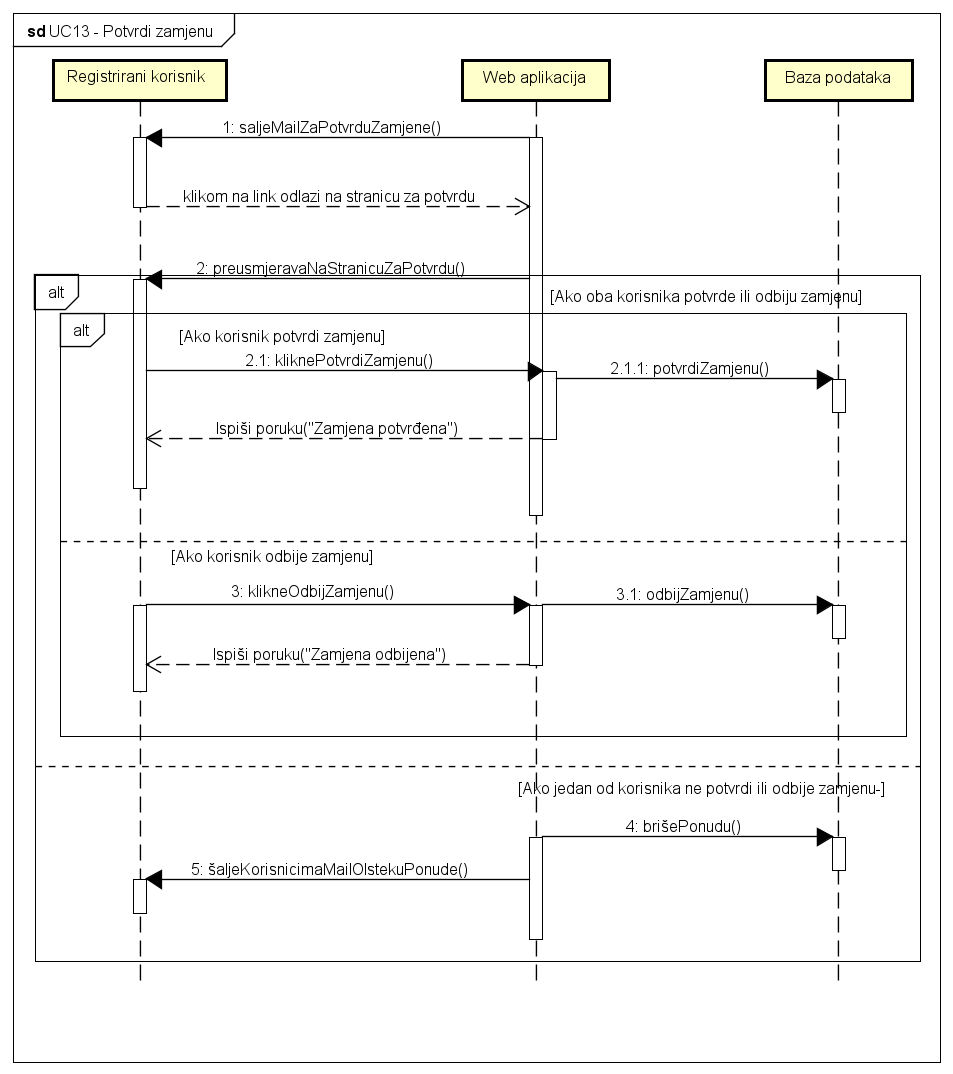
\includegraphics[width=.9\linewidth]{slike/UC13_sekvencijski_dijagram.PNG} 
		\centering
		\caption{Sekvencijski dijagram za UC13}
		\label{fig:sekvdij2}
	\end{figure}


\eject

\section{Ostali zahtjevi}

	\begin{itemize}
		\item 	\textit Sustav treba omoguciti rad više korisnika u stvarnom vremenu
		\item 	\textit Aplikacija treba biti prilagođena (engl. responsive) mobilnom uređaju
		\item 	\textit Korisničko sučelje i sustav moraju podržavati hrvatsku abecedu (dijakritičke znakove) prilikom unosa i prikaza tekstualnog sadržaja
		\item 	\textit Izvršavanje dijela programa u kojemu se pristupa bazi podataka ne smije trajati duže od nekoliko sekundi
		\item 	\textit Sustav treba biti implementiran kao web aplikacija koristeći objektrno-orijentirane jezike
		\item 	\textit Neispravno korištenje korisničkog sučelja ne smije narušiti funkcionalnost i rad sustava
		\item 	\textit Sustav treba biti jednostavan za korištenje, korisnici se moraju znati koristiti sučeljem bez opširnih uputa
		\item 	\textit Veza s bazom podataka mora biti kvalitetno zaštičena, brza i otporna na vanjske greške
		\item 	\textit Pristup sustavu mora biti omogućen iz javne mreže 
	\end{itemize}


	\chapter{Arhitektura i dizajn sustava}
		
		Pri razvoju web aplikacije Zamjena soba koristi se stil višeslojne arhitekture (engl. multi-layer architecture). To znači da uključuje više logičkih slojeva implementacije programske potpore. Općenito, osnova svih višeslojnih stilova je troslojni stil arhitekture koji sadrži:
		\begin{itemize}
		\item 	korisnički ili prezentacijski sloj (engl. presentation layer) – sloj s korisničkim sučeljem, odnosno onaj koji korisnik vidi i koji mu služi za unos podataka; uneseni podaci se mogu pohraniti u bazu ili u datotečni sustav
		\item 	sloj poslovne logike (engl. logic layer) – sloj s implementacijom poslovnih procesa i izračuna; pomoću njega se odvija sva komunikacija s bazom; on obrađuje i generira dinamički sadržaj 
		\item 	podatkovni sloj (engl. data layer) – sloj za pohranu podataka u bazu ili u datotečni sustav.
		\end{itemize}
		
		No,  klijentsku i poslužiteljsku stranu moguće je organizirati u više slojeva, pri čemu svaki sloj pruža uslugu nekom drugom.
	U slučaju naše aplikacije, u kojoj koristimo radni okvir Spring Boot, bilo je potrebno dodati više slojeva, te su slojevi arhitekture naše aplikacije:
		\begin{itemize}
		\item 	sloj korisničke strane – implementiran u JavaScriptu, koristi knjižnicu React koja omogućuje prikaz korisničkog sučelja. Pisan je u radnoj okolini Microsoft Visual Studio Code.
		\item 	sloj nadglednika (engl. controller) – povezuje korisničku stranu s poslužiteljskom stranom.
		\item 	sloj usluge (engl. service) – obavlja svu poslovnu logiku i potrebne izračune.
		\item 	sloj domene (engl. domain) – ima razrađeni model podataka domene
		\item 	sloj za pristup podatcima (engl. data access object, DAO) – omogućuje spremanje i dohvat podataka iz baze podataka te razmjenu tih podataka sa slojem domene
		\item 	sloj baze podataka – omogućuje pohranu podataka u relacijsku bazu PostgreSQL
	\end{itemize}
		
		
		Svi slojevi osim prvog i zadnjeg, pisani su na radnoj platformi Eclipse u programskom jeziku Java.
		\newline
		\hspace* {8mm} Primijetimo da slojevi naglednika, usluge i domene su analogni MVC arhitekturi. Odnosno sloj domene (domain) predstavlja model, sloj usluge (service) predstavlja view, te sloj naglednika (controller) predstavlja controller.
		\newline
		\hspace* {8mm} Izabrali smo baš tu arhitekturu kako bismo mogli bolje podijeliti rad među članovima tima (princip podijeli pa vladaj).
		\newline
		\hspace* {8mm} Nakon stavljanja aplikacije na server pomoću platforme Heroku, web poslužitelj je taj koji isporučuje sadržaj web aplikacije. To izvršava preko HTTP protokola na portu 8080.
		\newline
		\hspace* {8mm} Komunikacija među slojevima izvršava se u pozadini putem određenih portova (vrata). Sloj korisničke strane povezan je sa slojem nadglednika preko aplikacijskog programskog sučelja (API) na portu 3000. Sloj nadglednika, usluge i domene te sloj za pristup podacima su zajedno integrirani, odnosno povezuje ih radni okvir Spring Boot. Naposlijetku, sloj za pristup podacima je povezan sa slojem baze podataka preko porta 5432.
		
		
		

				
		\section{Baza podataka}
			
			
		\hspace{10mm} Koristi se relacijska baza podataka, ona se sastoji od skupa povezanih tablica odnosno relacija. Izabrali smo DBMS (database management system) PostgreSQL.
		\newline
		Entiteti baze su:
		\begin{itemize}
		\item \textit{student}
		\item \textit{sc}
		\item \textit{dom}
		\item \textit{menza}
		\item \textit{soba}
		\item \textit{filter}
		\item \textit{grad}
		\item \textit{oglas}
		\item \textit{lajkani\textunderscore oglas}
		\item \textit{moguca\textunderscore zamjena}
		\item \textit{zakljucane\textunderscore zamjene}
		\end{itemize}
		
			\subsection{Opis tablica}
			

				\hspace{10mm} \textbf{Student}
				\newline
				- u ovoj tablici se nalazi popis svih studenata i djelatnika studentskih centara.
				\newline
				\textit{Primarni ključ: id}
				
				
				\begin{longtabu} to \textwidth {|X[8, l]|X[6, l]|X[20, l]|}
					
					\hline \multicolumn{3}{|c|}{\textbf{student}}	 \\[3pt] \hline
					\endfirsthead
					
					\hline \multicolumn{3}{|c|}{\textbf{student}}	 \\[3pt] \hline
					\endhead
					
					\hline 
					\endlastfoot
					
					\cellcolor{LightGreen} id & BIGINT	&  	svakom korisniku se automatski generira id (identifikacijski broj)	\\ \hline
					username	& VARCHAR &  korisnik ga sam odabire, jedinstven je 	\\ \hline 
					email & VARCHAR & email korisnika, jedinstven je  \\ \hline 
					JMBAG & VARCHAR	& JMBAG korisnika		\\ \hline 
					name & VARCHAR	&  ime i prezime korisnika		\\ \hline 
					user\textunderscore role & INT	& sustav dodijeljuje ovlasti kako bi razlikovao studente od SC djelatnika		\\ \hline 
					password & VARCHAR	&  hash lozinke		\\ \hline 
					locked & BOOLEN	&  osposobljenost ili neosposobljenost korisnikovog računa		\\ \hline 
					enabled & BOOLEAN	&  aktiviranost ili deaktiviranost korisnikovog računa		\\ \hline 
					potvrdjeni\textunderscore lanac & BIGINT	&  id lanca u kojem je potvrđen, dog ga nema vrijednost mu je null		\\ \hline 
					
					
				\end{longtabu}
				
				
				\textbf{Studentski centar}
				\newline
				\textit{Primarni ključ: idSC}
				\newline
				\textit{Strani ključ: grad\textunderscore id\textunderscore grada}
				\newline
				
				
				\begin{longtabu} to \textwidth {|X[6, l]|X[6, l]|X[20, l]|}
					
					\hline \multicolumn{3}{|c|}{\textbf{SC}}	 \\[3pt] \hline
					\endfirsthead
					
					\hline \multicolumn{3}{|c|}{\textbf{SC}}	 \\[3pt] \hline
					\endhead
					
					\hline 
					\endlastfoot
					
					\cellcolor{LightGreen}idSC & BGIINT	&  	svakom studentskom centru se automatski dodjeljuje id	\\ \hline
					ime	& VARCHAR & naziv studentskog centra  	\\ \hline 
					grad\textunderscore id\textunderscore grada & INT & grad u kojem se nalazi studentski centar  \\ \hline 
					
					
					
				\end{longtabu}
				
				
				
				
				\textbf{Dom}
				\newline
				\textit{Primarni ključ: id\textunderscore dom}
				\newline
				\textit{Strani ključ: menza\textunderscore naziv\textunderscore menze, sc\textunderscore idsc, grad\textunderscore id\textunderscore grada}
				\newline
			
				
				\begin{longtabu} to \textwidth {|X[14, l]|X[6, l]|X[20, l]|}
					
					\hline \multicolumn{3}{|c|}{\textbf{dom}}	 \\[3pt] \hline
					\endfirsthead
					
					\hline \multicolumn{3}{|c|}{\textbf{dom}}	 \\[3pt] \hline
					\endhead
					
					\hline 
					\endlastfoot
					
					\cellcolor{LightGreen}id\textunderscore dom & BIGINT	&  	svakom studentskom domu se automatski dodjeljuje id	\\ \hline
					ime<c doma	& VARCHAR & naziv doma  	\\ \hline 
					grad\textunderscore id\textunderscore grada & INT & grad u kojem se dom nalazi  \\ \hline 
					najbliza\textunderscore menza\textunderscore naziv\textunderscore menze & VARCHAR	&  naziv najblize menze		\\ \hline 
					\cellcolor{LightBlue}sc\textunderscore idSC	& BIGINT &  id studentskog centra u kojem se nalazi 	\\ \hline 
					
					
				\end{longtabu}
				
				
				\textbf{Menza}
				\newline
				- najbliža menza studentskom domu
				\newline
				\textit{Primarni ključ: naziv\textunderscore menze}
				\newline
				\textit{Strani ključ: grad\textunderscore id\textunderscore grada}
				
				
				
				\begin{longtabu} to \textwidth {|X[6, l]|X[6, l]|X[20, l]|}
					
					\hline \multicolumn{3}{|c|}{\textbf{menza}}	 \\[3pt] \hline
					\endfirsthead
					
					\hline \multicolumn{3}{|c|}{\textbf{menza}}	 \\[3pt] \hline
					\endhead
					
					
					\cellcolor{LightGreen}naziv\textunderscore menze & VARCHAR	&  	naziv menze	\\ \hline
					grad\textunderscore id\textunderscore grada	& INT & id grada u kojem se nalazi  	\\ \hline 
					
					
					
				\end{longtabu}
				
				
				\textbf{Soba}
				\newline
				- studentova sobe
				\newline
				\textit{Primarni ključ: id\textunderscore soba}
				\newline
				\textit{Strani ključ: id\textunderscore doma\textunderscore id\textunderscore dom, id\textunderscore studenta\textunderscore id}
				
				
				
				\begin{longtabu} to \textwidth {|X[8, l]|X[6, l]|X[20, l]|}
					
					\hline \multicolumn{3}{|c|}{\textbf{soba}}	 \\[3pt] \hline
					\endfirsthead
					
					\hline \multicolumn{3}{|c|}{\textbf{soba}}	 \\[3pt] \hline
					\endhead
					
					\hline 
					\endlastfoot
					
					\cellcolor{LightGreen}id\textunderscore soba & BIGINT	&  	svakoj sobi se automatski dodjeljuje jedinstveni id	\\ \hline
					kat	& SMALLINT & kat na kojem se nalazi  	\\ \hline 
					kategorija\textunderscore sobe	& SMALLINT & kategorija sobe studentskog doma (od 1 do 7)  	\\ \hline 
					paviljon	& SMALLINT & paviljon u kojem se nalazi  	\\ \hline
					id\textunderscore doma\textunderscore id\textunderscore dom	& BIGINT & id doma u kojem se nalazi  	\\ \hline
					id\textunderscore studenta\textunderscore id	& BIGINT & id studenta koji raspolaže tom sobom  	\\ \hline 
					
					
					
				\end{longtabu}
				
				
				\textbf{Filter}
				\newline
				- služi za filtriranje oglasa na početnoj stranici
				\newline
				\textit{Primarni ključ: id\textunderscore filter}
				\newline
				\textit{Strani ključ: id\textunderscore doma\textunderscore id\textunderscore dom, id\textunderscore studenta\textunderscore id}
				
				
				
				\begin{longtabu} to \textwidth {|X[8, l]|X[6, l]|X[20, l]|}
					
					\hline \multicolumn{3}{|c|}{\textbf{filter}}	 \\[3pt] \hline
					\endfirsthead
					
					\hline \multicolumn{3}{|c|}{\textbf{filter}}	 \\[3pt] \hline
					\endhead
					
					\hline 
					\endlastfoot
					
					\cellcolor{LightGreen}id\textunderscore filter & BIGINT	&  	svakome filteru se automatski dodjeljuje jedinstveni id	\\ \hline
					kat	& SMALLINT & kat koji se pretražuje  	\\ \hline 
					kategorija\textunderscore sobe	& SMALLINT & kategorija sobe koja se pretražuje  	\\ \hline 
					paviljon	& SMALLINT & paviljon koji se pretražuje  	\\ \hline
					id\textunderscore doma\textunderscore id\textunderscore dom	& BIGINT & id doma koji se pretražuje  	\\ \hline
					student\textunderscore id	& BIGINT & id studenta koji koji je napravio filter  	\\ \hline 
					
					
					
				\end{longtabu}
				
				
				\textbf{Grad}
				\newline
				\textit{Primarni ključ: id\textunderscore grada}
				
				
				
				\begin{longtabu} to \textwidth {|X[6, l]|X[6, l]|X[20, l]|}
					
					\hline \multicolumn{3}{|c|}{\textbf{grad}}	 \\[3pt] \hline
					\endfirsthead
					
					\hline \multicolumn{3}{|c|}{\textbf{grad}}	 \\[3pt] \hline
					\endhead
					
					\hline 
					\endlastfoot
					
					\cellcolor{LightGreen}id\textunderscore grada & INT	&  	svakome gradu se automatski dodjeljuje jedinstveni id	\\ \hline
					ime\textunderscore grada	& VARCHAR & naziv grada  	\\ \hline 
					
					
					
				\end{longtabu}
				
				
				\textbf{Oglas}
				\newline
				- oglas kojime student nudi svoju sobu
				\newline
				\textit{Primarni ključ: id\textunderscore oglas}
				\newline
				\textit{Strani ključ: dom\textunderscore id\textunderscore dom, student\textunderscore id}
				
				
				\begin{longtabu} to \textwidth {|X[7, l]|X[6, l]|X[20, l]|}
					
					\hline \multicolumn{3}{|c|}{\textbf{oglas}}	 \\[3pt] \hline
					\endfirsthead
					
					\hline \multicolumn{3}{|c|}{\textbf{oglas}}	 \\[3pt] \hline
					\endhead
					
					\hline 
					\endlastfoot
					
					\cellcolor{LightGreen}id\textunderscore oglas & BIGINT	&  	svakome oglasu se automatski dodjeljuje jedinstveni id	\\ \hline
					aktivan	& BOOLEAN & student može deaktivirati aktivan oglas  	\\ \hline 
					kat	& SMALLINT & kat na kojem se nalazi studentova soba  	\\ \hline 
					kategorija\textunderscore sobe	& SMALLINT & kategorija studentove sobe  	\\ \hline 
					paviljon	& SMALLINT & paviljon u kojem se nalazi studentova soba  	\\ \hline
					dom\textunderscore id\textunderscore dom	& BIGINT & id doma u kojem se nalazi studentova soba  	\\ \hline
					student\textunderscore id	& BIGINT & id studenta koji je sastavio oglas  	\\ \hline 
					
					
					
				\end{longtabu}
				
				
				\textbf{Lajkani oglas}
				\newline
				- lajkovi koji povezuju studenta i oglas koji je on lajkao
				\newline
				\textit{Primarni ključ: oglas\textunderscore id, student\textunderscore id}
				
				
				\begin{longtabu} to \textwidth {|X[7, l]|X[6, l]|X[20, l]|}
					
					\hline \multicolumn{3}{|c|}{\textbf{lajkani\textunderscore oglas}}	 \\[3pt] \hline
					\endfirsthead
					
					\hline \multicolumn{3}{|c|}{\textbf{lajkani\textunderscore oglas}}	 \\[3pt] \hline
					\endhead
					
					\hline 
					\endlastfoot
					
					\cellcolor{LightGreen}oglas\textunderscore id & BIGINT	&  	id lajkanog oglasa	\\ \hline
					\cellcolor{LightBlue}student\textunderscore id & BIGINT	&  	id studenta koji je lajkao oglas	\\ \hline
					stupanj\textunderscore lajkanja	& INT & Može biti: 1, 2 ili 3 ovisno o pritisutom broju srca. Također može biti 0 za uklananje lajka te 4 za opciju "ne prikazuj više"  	\\ \hline 
					procitano	& BOOLEAN & Služi za obavještavanje autora oglasa o novim dobivenim lajkovima  	\\ \hline 
					
					
				\end{longtabu}
				
				
				\textbf{Moguća zamjena}
				\newline
				- služi za prikaz ostvarivih zamjena korisniku
				\newline
				\textit{Primarni ključ: id\textunderscore lanca, redni\textunderscore broj}
				\newline
				\textit{Strani ključ: oglas\textunderscore id\textunderscore oglas}
				
				
				\begin{longtabu} to \textwidth {|X[6, l]|X[6, l]|X[20, l]|}
					
					\hline \multicolumn{3}{|c|}{\textbf{moguca\textunderscore zamjena}}	 \\[3pt] \hline
					\endfirsthead
					
					\hline \multicolumn{3}{|c|}{\textbf{moguca\textunderscore zamjena}}	 \\[3pt] \hline
					\endhead
					
					\hline 
					\endlastfoot
					
					\cellcolor{LightGreen}id\textunderscore lanca & BIGINT	&  	svakome lancu zamjena se automatski dodjeljuje jedinstveni id	\\ \hline
					\cellcolor{LightBlue}redni\textunderscore broj & SMALLINT	&  	Redni broj oglasa u lancu zamjena 	\\ \hline
					oglas\textunderscore id\textunderscore oglas	& BIGINT & id oglasa studentovog oglasa u lancu zamjena	\\ \hline 
					procitano	& BOOLEAN & Služi za obavještavanje autora oglasa o novim mogućim zamjenama  	\\ \hline 
					
					
				\end{longtabu}
				
				
				
				\textbf{Zaključane zamjene}
				\newline
				- potvrđene zamjene soba od strane studenata, koje se prikazuju djelatnku studentskog centra
				\newline
				\textit{Primarni ključ: id\textunderscore zamjene}
				\newline
				\textit{Strani ključ: oglas1\textunderscore id\textunderscore oglas, oglas2\textunderscore id\textunderscore oglas}
				
				
				\begin{longtabu} to \textwidth {|X[7, l]|X[6, l]|X[20, l]|}
					
					\hline \multicolumn{3}{|c|}{\textbf{zakljucane\textunderscore zamjene}}	 \\[3pt] \hline
					\endfirsthead
					
					\hline \multicolumn{3}{|c|}{\textbf{zakljucane\textunderscore zamjene}}	 \\[3pt] \hline
					\endhead
					
					
					\hline 
					\endlastfoot
					
					id\textunderscore zamjene & BIGINT	&  	svakoj zaključanoj zamjeni se automatski dodjeljuje jedinstveni id	\\ \hline
					aktivan & BOOLEAN	&  	izvršenost zamjene	\\ \hline
					oglas1\textunderscore id\textunderscore oglas	& BIGINT & id oglasa 1 u zamjeni  	\\ \hline 
					oglas2\textunderscore id\textunderscore oglas	& BIGINT & id oglasa 2 u zamjeni  	\\ \hline
					
				\end{longtabu}
				
				\eject
				
				
			
			\subsection{Dijagram baze podataka}
			Priložen je ER-model (entity realtionship model) baze podataka. Strani ključevi su prikazani crtom među tablicama. Plava točka označava da u toj tablici se nalazi strani ključ koji je u povezanoj tablici primarni ključ.
			\newline
			
			\begin{figure}[H]
			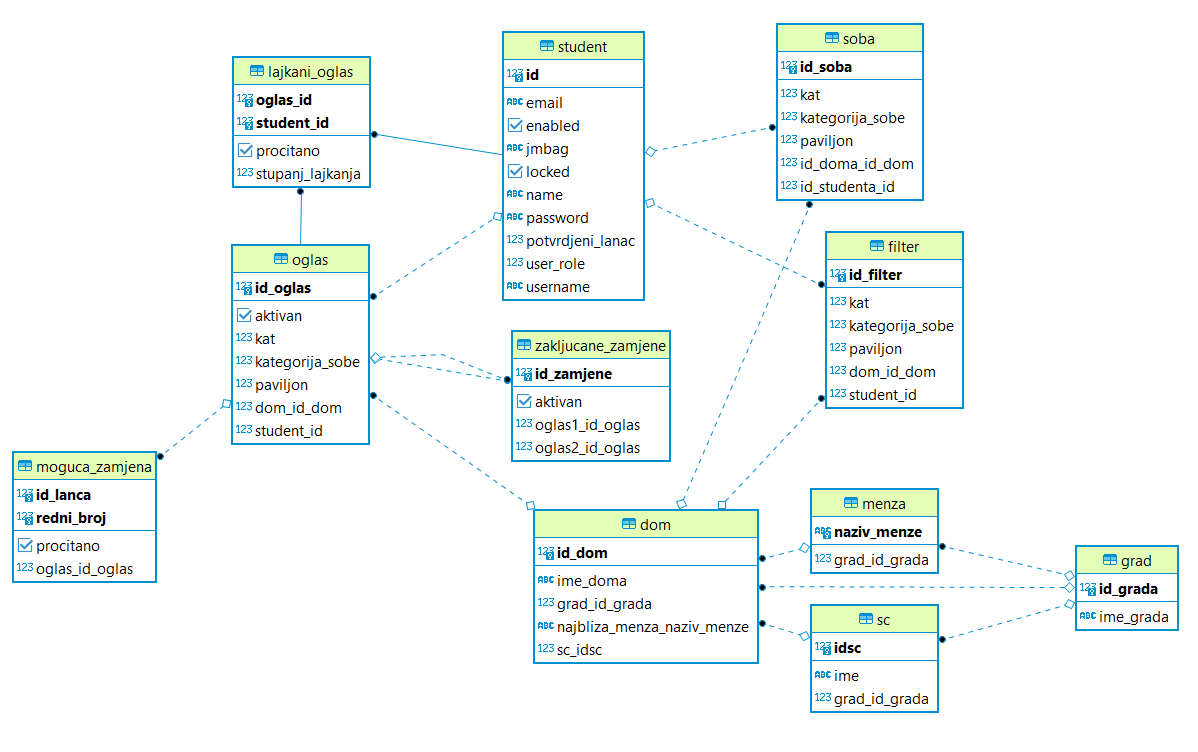
\includegraphics[scale=0.7]{slike/novi_er_model.png} 
			\centering
			\caption{Dijagram baze podataka}
			\label{fig:baza}
		\end{figure}
		
\eject
			
			
			
		\section{Dijagram razreda}
		
		Na slici 4.1 je prikazan potupuni dijagram razreda. Stavke su grupirane prema odgovarajućem paketu unutar kojeg se nalaze. Zbog lakšeg prikaza, kružićima su označena sučelja.
		\newline
		JWT (JSON Web Token) služi za identifikaciju korisnika. On dodjeljuje token svakom korisniku. Preko toga se svi korisnikovi zahtjevi mogu ispuniti u web aplikaciji.
		
		\begin{figure}[H]
			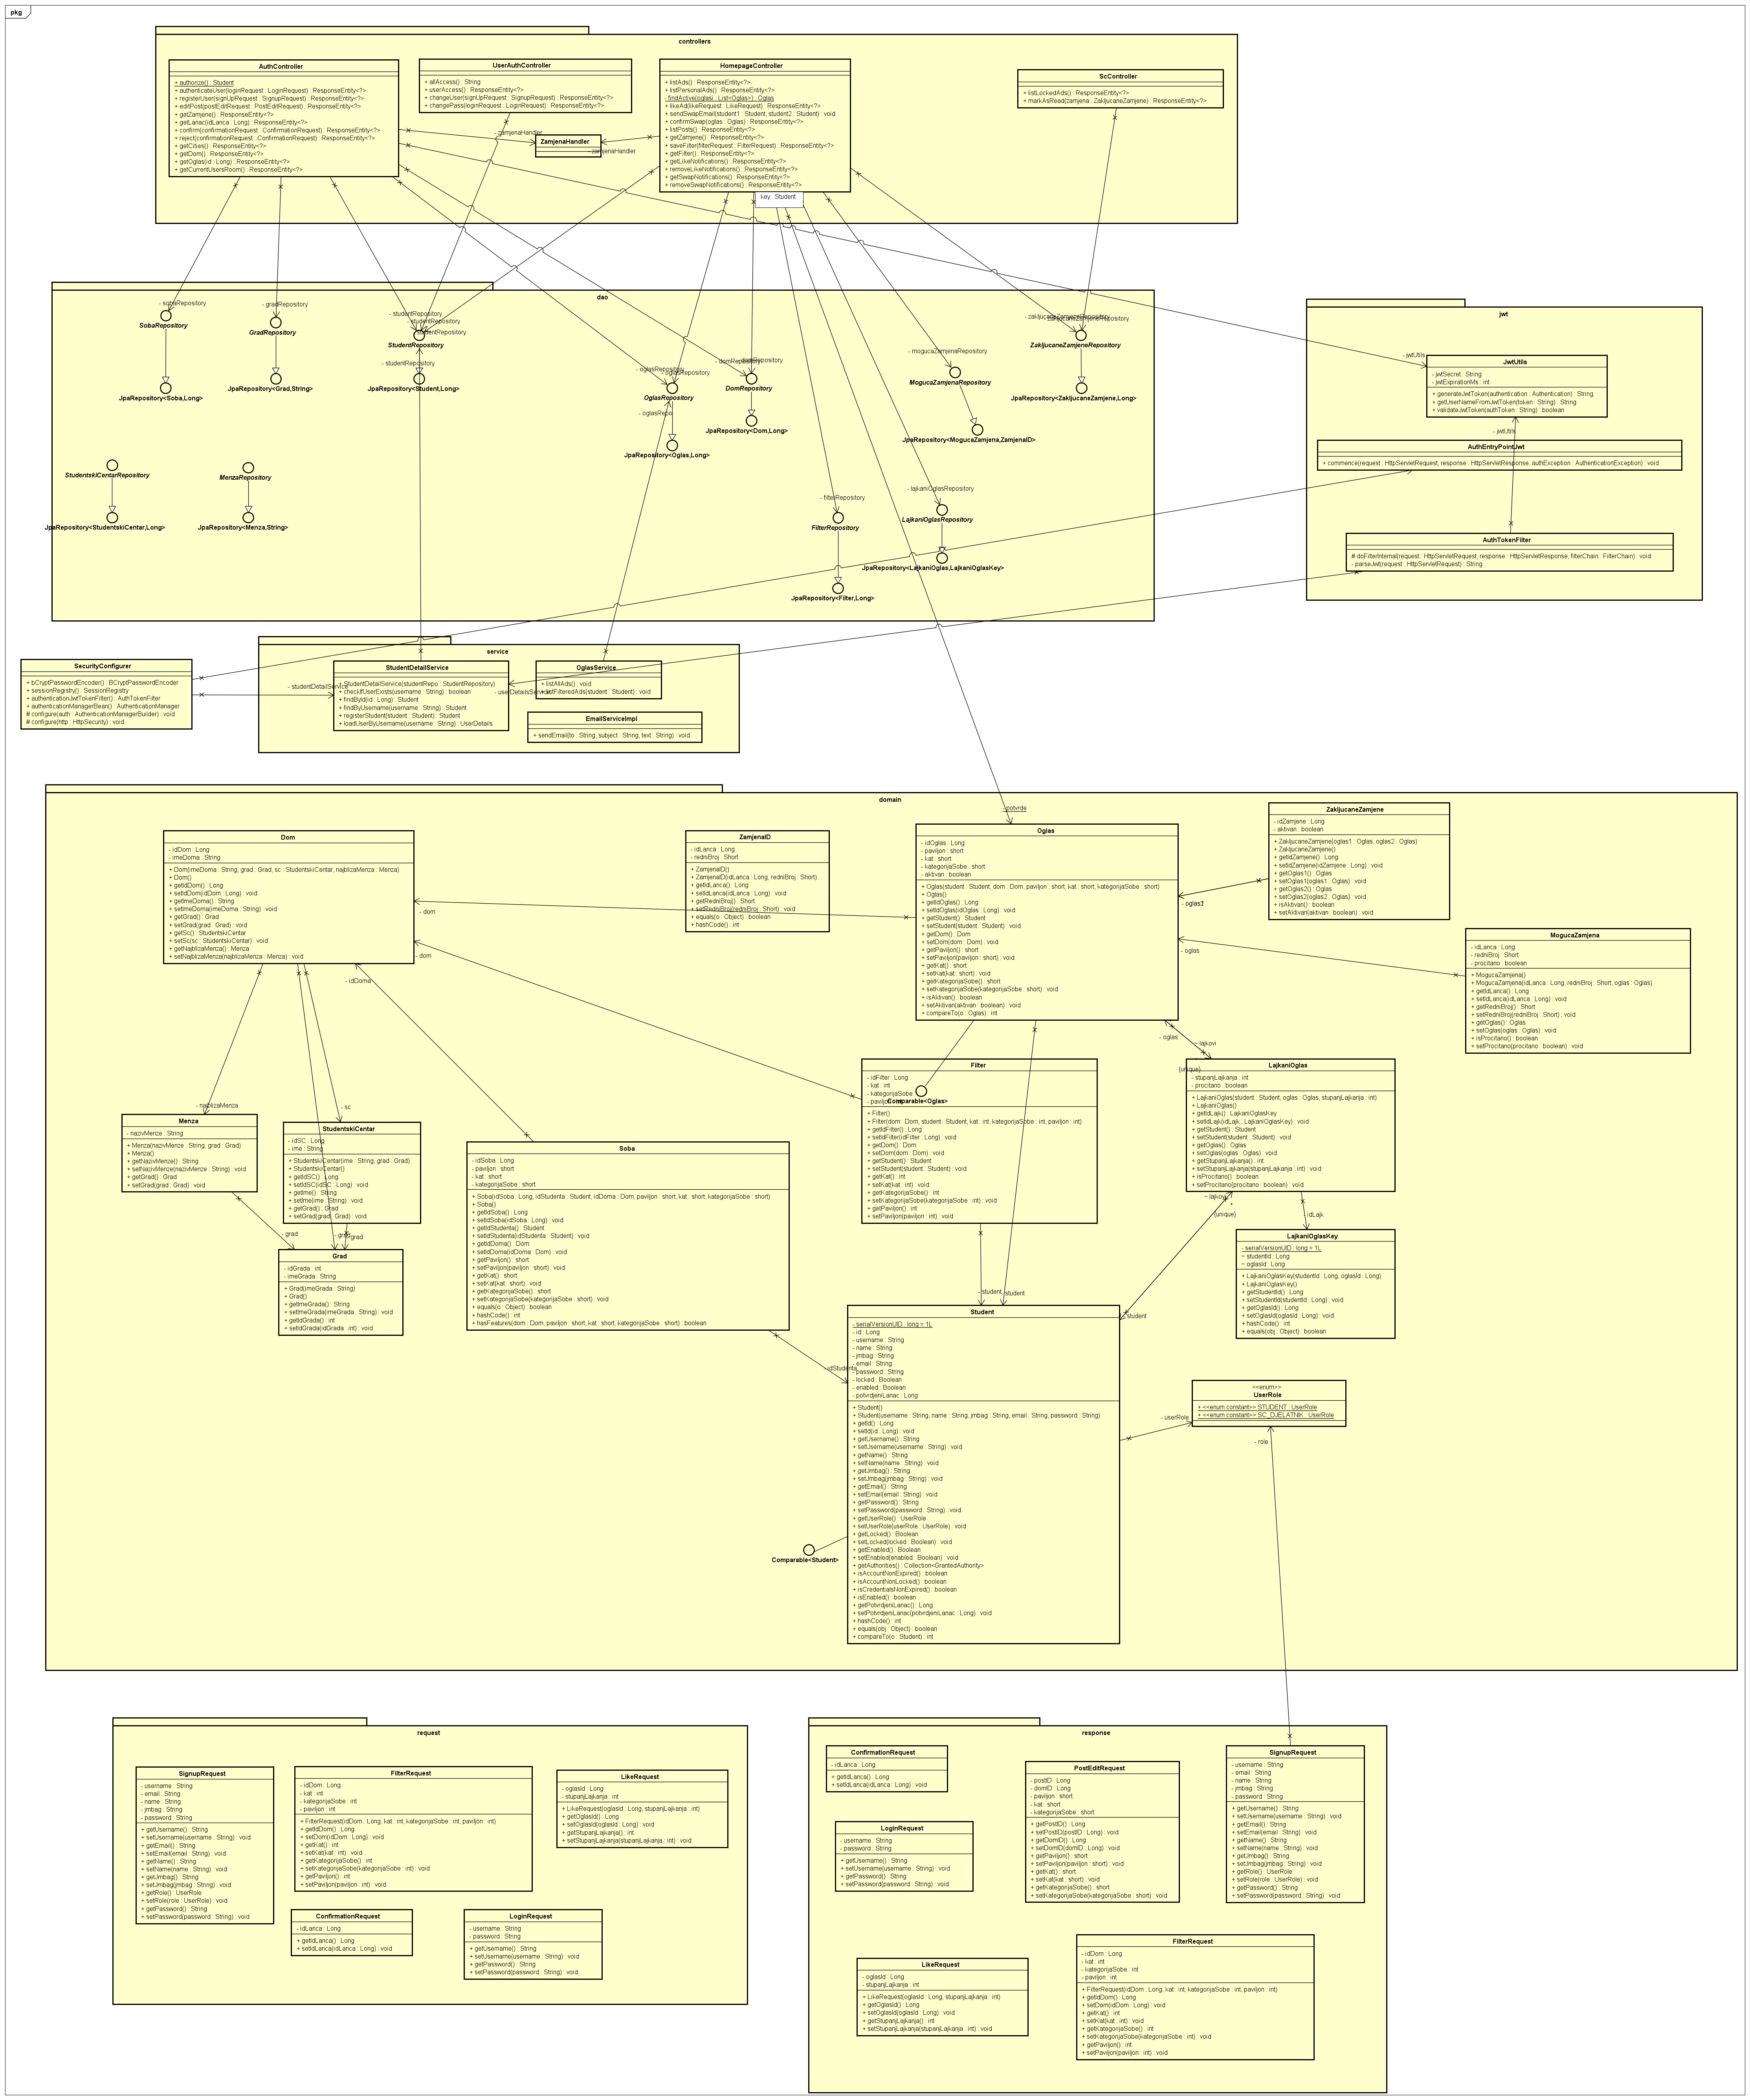
\includegraphics[scale=0.15]{slike/dijag_raz.png} 
			\centering
			\caption{Dijagram razreda}
			\label{fig:models}
		\end{figure}
		
		\eject
			
			\section{Dijagram stanja}
			
				\textbf{\textit{}}\\
			
Dijagram stanja prikazuje stanja objekta te prijelaze iz jednog stanja u drugo te-
meljene na dogadajima. Na slici 4.6 prikazan je dijagram stanja za registriranog
korisnika. Nakon prijave, klijentu se prikazuje pocetna stranica na kojoj može pregledati oglase te poželji filtrirati oglase.
Odabrani oglas korisnik može i lajkati. Korisnik može odabirom različitih opcija i urediti vlastiti profil, pregledati predane oglase, stvoriti novi oglas i urediti predani oglas, pregledati oglase osoba koji su lajkali korisnikov oglas (odabirom opcije "Dobiveni lajkovi"). Ukoliko korisnik odabere opciju "Moguće zamjene", može vidjeti sve oglase koji mu se nude za zaključavanje zamjene te zaključati zamjenu.

			\begin{figure}[H]
				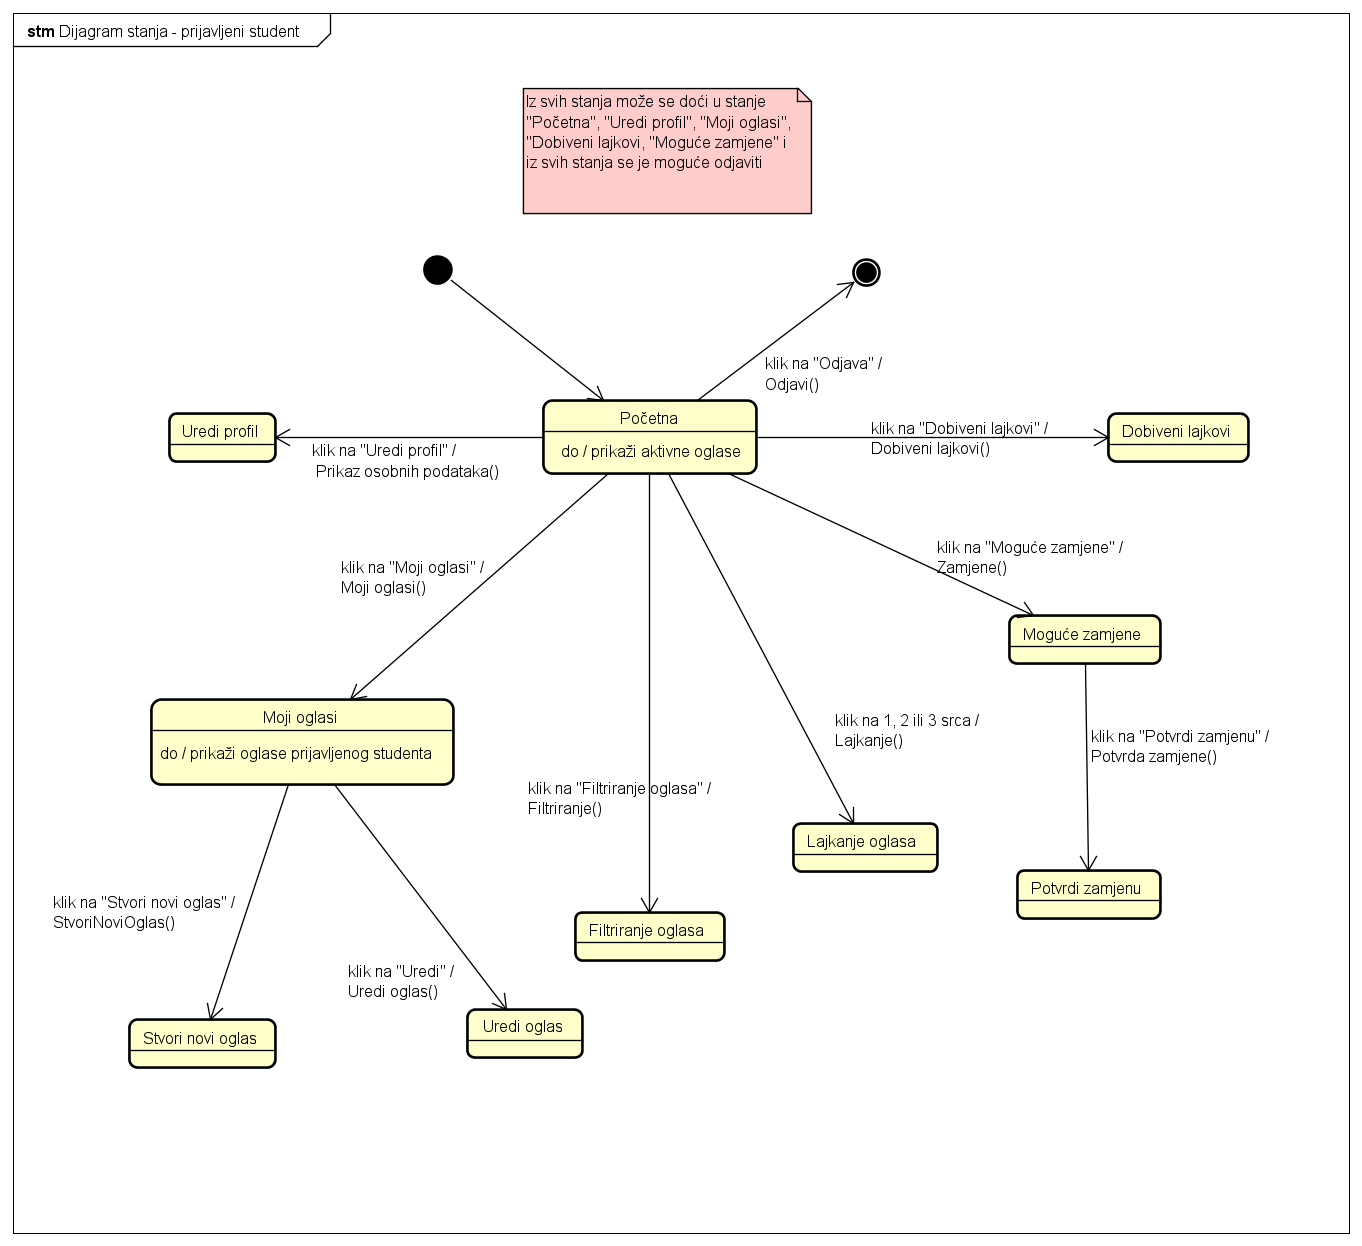
\includegraphics[scale=0.3]{slike/Dijagram_stanja_prijavljeni_student.PNG} %veličina slike u odnosu na originalnu datoteku i pozicija slike
				\centering
				\caption{Dijagram stanja}
				\label{fig:dijagramStanja}
			\end{figure}
			
			
			\eject 
			
			\section{Dijagram aktivnosti}
			
			\textbf{\textit{}}\\
			
			Dijagram aktivnosti primjenjuje se za opis modela toka upravljanja ili toka po-
dataka. Ne upotrebljava se za modeliranje dogadajima poticanog ponasanja. U 
modeliranju toka upravljanja svaki novi korak poduzima se nakon završenog prethodnog, a naglasak je na jednostavnosti. Na dijagramu aktivnosti 4.7 prikazan je
proces lajkanja oglasa. Korisnik nakon prijave u sustav ima uvid u predane oglase. On zatim može odabrati i lajkati neki od prikazanih oglasa ili unijeti filtere za pretraživanje oglasa. Ukoliko korisnik odabere opciju za filtriranje oglasa, sustav će mu prikazati samo one oglase koji odgovaraju njegovim kriterijima te korisnik onda po želji lajka. Nakon što korisnik lajka oglas, promjene se unose u sustav i korisniku se prokazuje uspješno lajkanje u obliku obojanih srca koji su ranije bili bijeli.
			
			\begin{figure}[H]
				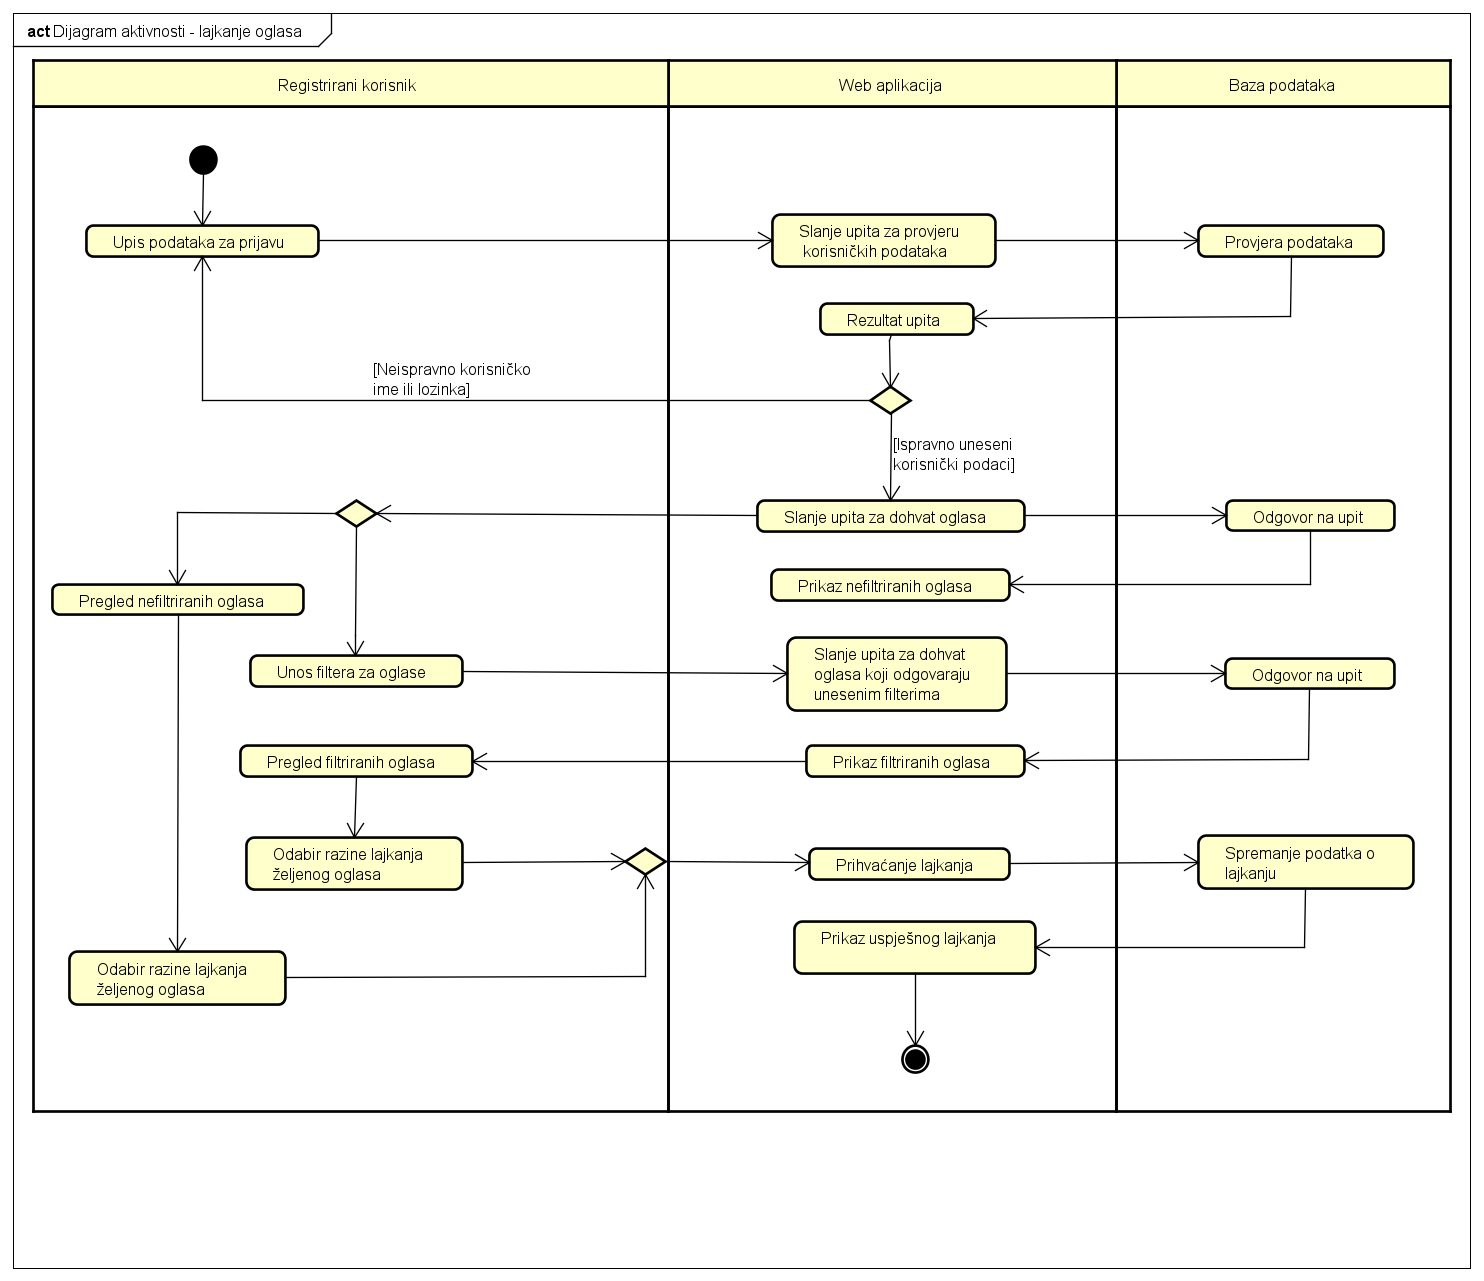
\includegraphics[scale=0.4]{slike/dijagram_ativnosti.PNG} %veličina slike u odnosu na originalnu datoteku i pozicija slike
				\centering
				\caption{Dijagram aktivnosti}
				\label{fig:dijagramAktivnosti}
			\end{figure}
			
			
			\eject
			
			\section{Dijagram komponenti}
			
			Dijagram komponenti prikazan na slici 4.8 opisuje organizaciju i međuovisnost
komponenti, interne strukture i odnose prema okolini. Sustavu se pristupa preko
dva različita sučelja. Preko sučelja za dohvat HTML, CSS i JS datoteka poslužuju se datoteke koje pripadaju frontend dijelu aplikacije. Router je komponenta koja na
upit s url odreduje koja datoteka ce se poslužiti na sučelje. Frontend dio se sastoji
od niza JavaScript datoteka koje su raspoređene u logičke cjeline nazvane po tipovima aktora koji im pristupaju. Sve JavaScript datoteke ovise o React biblioteci iz
koje dohvacaju gotove komponente kao što su gumbi, forme i slično. Preko sučelja za dohvat JSON podataka pristupa se REST API komponenti. REST API poslužuje podatke koji pripadaju backend dijelu aplikacije. EntityFrameworkCore je zadužen za dohvaćanje tablica iz baze podataka pomoću SQL upita. Reactview komponenta preko dostupnih sučelja komunicira s aplikacijom te ovisno o korisnikovim akcijama osvježava prikaz i dohvaća nove podatke ili datoteke.

			
			\begin{figure}[H]
				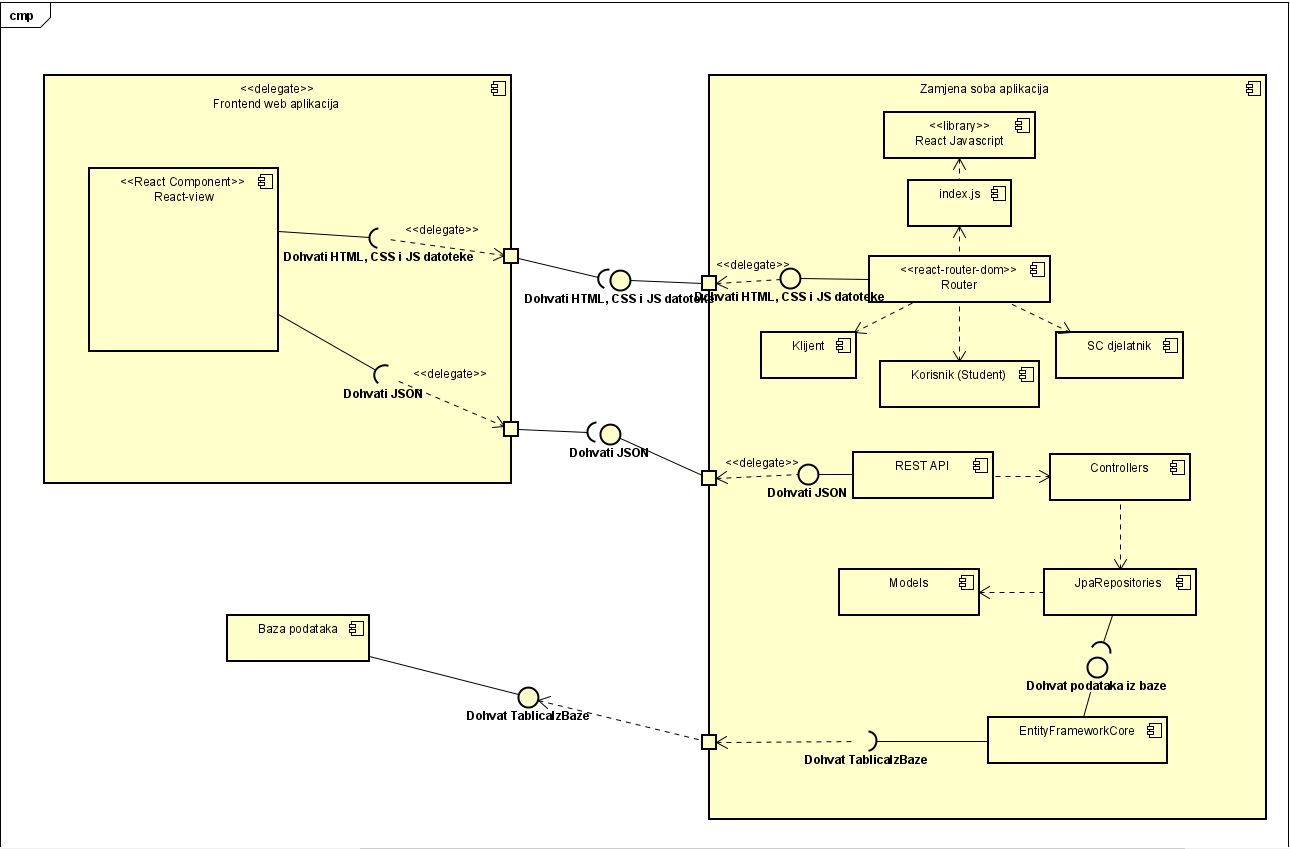
\includegraphics[scale=0.4]{slike/dijagram_komponenti.png} %veličina slike u odnosu na originalnu datoteku i pozicija slike
				\centering
				\caption{Dijagram komponenti}
				\label{fig:dijagramKomponenti}
			\end{figure}
			
			\eject
			
			
			
			
	\chapter{Implementacija i korisničko sučelje}
		
		
		\section{Korištene tehnologije i alati}
		
		
			Komunikacija u timu ostvarena je pomoću aplikacija WhatsApp i Discord. Za upravljanje i verzioniranje izvornog koda korišten je Git te udaljeni repozitorij na web platformi GitLab.
			\vspace{3mm}
Za razvoj backenda kokrištena su razvojna okruženja (IDE) Eclipe i IntelliJ Idea, a za razvoj frontenda Visual Studio Code. Rad sa bazom podataka ostvaren je pomoću sustava PostgreSQL i pgAdmin. Aplikacija je napisana u programskim jezicima Java i JavaScript.
\vspace{3mm}
Backend aplikacije izrađen je u radnom okviru Spring Boot, koji sadrži brojne biblioteke za rad sa bazom podataka, izradu web aplikacije i sigurnost pri slanju HTTP zahtjeva. Za frontend je korištena biblioteka React koja se koristi za izgradnju korisničkih sučelja.
Aplikacija je hostana na cloud platformi Heroku. \\


\url{https://www.whatsapp.com} \\
\url{https://discord.com} \\
\url{https://git-scm.com} \\
\url{https://about.gitlab.com} \\
\url{https://www.eclipse.org/ide} \\
\url{https://www.jetbrains.com/idea} \\
\url{https://code.visualstudio.com} \\
\url{https://www.postgresql.org} \\
\url{https://www.java.com} \\
\url{https://www.javascript.com} \\
\url{https://spring.io} \\
\url{https://reactjs.org} \\
\url{https://www.heroku.com} \\
		
			\eject 
		
	
		\section{Ispitivanje programskog rješenja}
			
			Provedeno je automatizirano ispitivanje programskog rješenja. Testiranje komponenti sustava izvedeno je pomoću JUnit testova, a ispitivanje ponašanja sustava pomoću alata Selenium IDE.
	
			
			\subsection{Ispitivanje komponenti}
			Proveli smo 7 JUnit testova koji testiraju razrede i metode u aplikaciji.
			\vspace{3mm}
			
			\textbf{Ispitni slučaj 1: Prvi test testira registraciju novog usera u aplikaciji. }	
			
			\begin{figure}[H]
				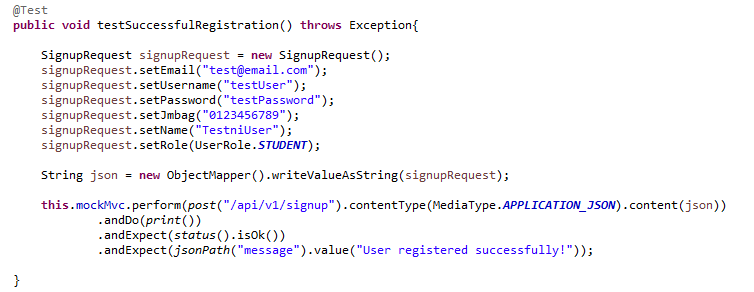
\includegraphics[scale=0.9]{slike/test1.PNG} %veličina slike u odnosu na originalnu datoteku i pozicija slike
				\centering
				\label{fig:test1}
			\end{figure}
			
			\textbf{Ispitni slučaj 2 i 3: Sljedeća dva testa testiraju hoće li se dogoditi iznimka u slučaju ako pokušamo 
registrirati novog korisnika u sustav ukoliko već postoji korisnik s istim usernameom ili se email 
već koristi.
}	
			
			\begin{figure}[H]
				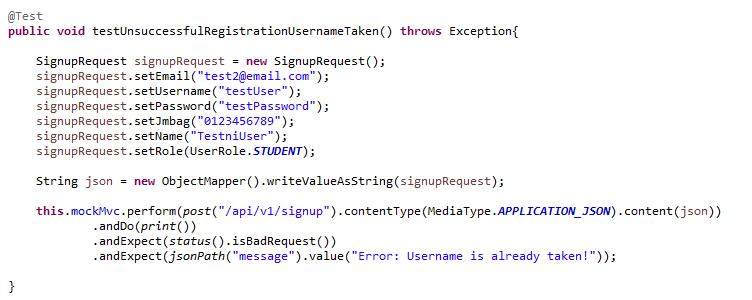
\includegraphics[scale=0.9]{slike/test2.PNG} %veličina slike u odnosu na originalnu datoteku i pozicija slike
				\centering
				\label{fig:test2}
			\end{figure}
			
			\begin{figure}[H]
				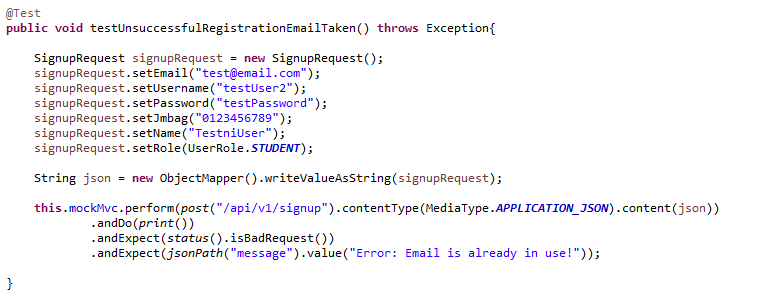
\includegraphics[scale=0.9]{slike/test3.PNG} %veličina slike u odnosu na originalnu datoteku i pozicija slike
				\centering
				\label{fig:test3}
			\end{figure}
			
			\textbf{Ispitni slučaj 4: Test 4 provjerava api koji vraća podatke o trenutačno logiranom korisniku.  }	
			
			\begin{figure}[H]
				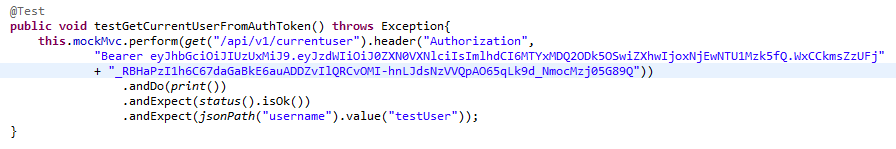
\includegraphics[scale=0.9]{slike/test4.PNG} %veličina slike u odnosu na originalnu datoteku i pozicija slike
				\centering
				\label{fig:test4}
			\end{figure}
			
			\textbf{Ispitni slučaj 5:Test 5 provjerava baca li se odgovarajuća iznimka kada se pokuša koristiti api za 
provjeru podataka o trenutačno logiranom korisniku, a odgovarajući JWT token nije bio poslan.}	
			
			\begin{figure}[H]
				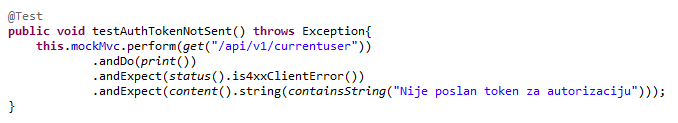
\includegraphics[scale=0.9]{slike/test5.PNG} %veličina slike u odnosu na originalnu datoteku i pozicija slike
				\centering
				\label{fig:test5}
			\end{figure}
			
			\textbf{Ispitni slučaj 6: Test 6 provodi provjeru logiranja u sustav. Ukoliko se korisnik uspješno ulogira, test prolazi.
}	
			
			\begin{figure}[H]
				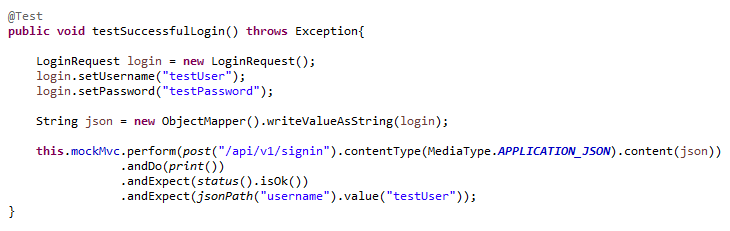
\includegraphics[scale=0.9]{slike/test6.PNG} %veličina slike u odnosu na originalnu datoteku i pozicija slike
				\centering
				\label{fig:test6}
			\end{figure}
			
			\textbf{Ispitni slučaj 7: Test 7 provjera što se će se dogoditi u slučaju neispravnih korisničkih podataka za login. 
Očekivano ponašanje je error kod 400 uz poruku "Bad credentials".
}	
			
			\begin{figure}[H]
				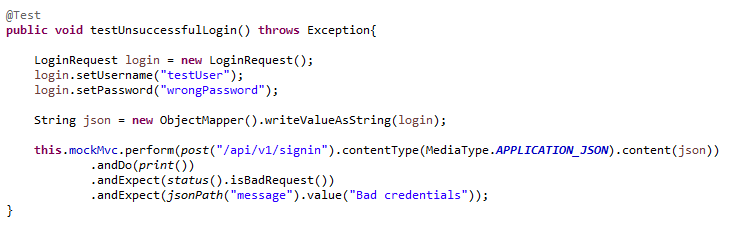
\includegraphics[scale=0.9]{slike/test7.PNG} %veličina slike u odnosu na originalnu datoteku i pozicija slike
				\centering
				\label{fig:test7}
			\end{figure}
			
			
			
			\subsection{Ispitivanje sustava}
			
			 Ispitivanje sustava provedeno je dodatkom za preglednik Selenium IDE. Testirani su slučajevi registracije, prijave korisnika, objave oglasa i oznake oglasa da se više ne prikazuje.
			 
			 \textbf{Ispitni slučaj 1:Registracija korisnika
}	
Testirana je registracija korisnika s jedinstvenim podatcima te je očekivani rezultat uspješna registracija.
			
			\begin{figure}[H]
				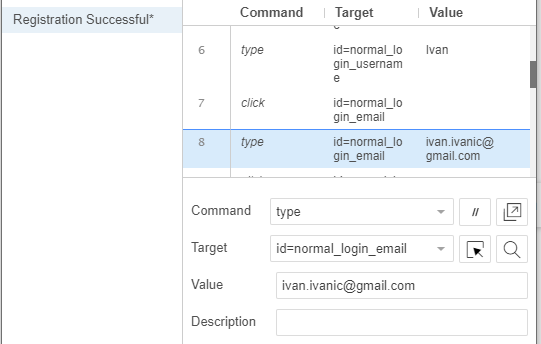
\includegraphics[scale=0.6]{slike/test8.PNG} %veličina slike u odnosu na originalnu datoteku i pozicija slike
				\centering
				\label{fig:test8}
			\end{figure}
			\begin{figure}[H]
				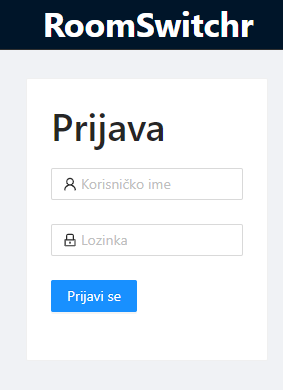
\includegraphics[scale=0.6]{slike/test8pom.PNG} %veličina slike u odnosu na originalnu datoteku i pozicija slike
				\centering
				\label{fig:test8pom}
			\end{figure}
			
			\textbf{Ispitni slučaj 2: Prijava nepostojećeg korisnika}	
			Testirana je prijava korisnika s nepostojećim korisničkim imenom te je očekivani rezultat odbijanje prijave i ispis poruke u grešci.
			
			\begin{figure}[H]
				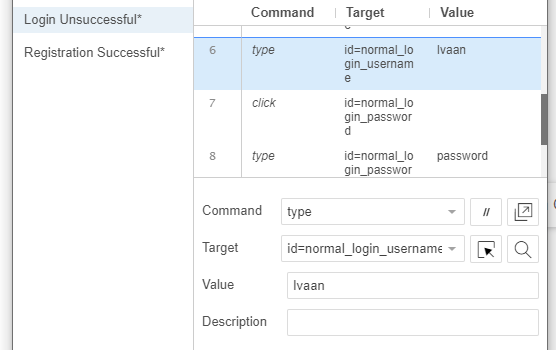
\includegraphics[scale=0.6]{slike/test9.PNG} %veličina slike u odnosu na originalnu datoteku i pozicija slike
				\centering
				\label{fig:test9}
			\end{figure}
			\begin{figure}[H]
				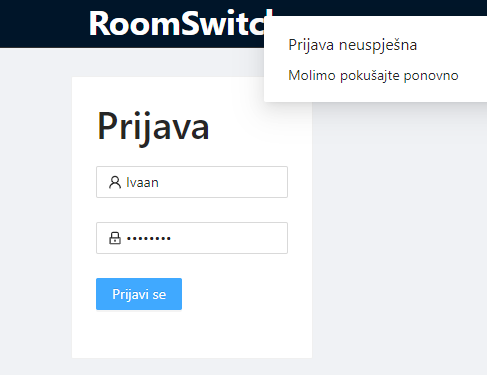
\includegraphics[scale=0.6]{slike/test9pom.PNG} %veličina slike u odnosu na originalnu datoteku i pozicija slike
				\centering
				\label{fig:test9pom}
			\end{figure}
			
			\textbf{Ispitni slučaj 3: Predaja oglasa}
			Testirana je predaja oglasa korisnika koji već ima aktivni oglas. Očekivani rezultat je stvaranje novog aktivnog oglasa, a prethodni aktivni oglas postaje neaktivan.	
			
			\begin{figure}[H]
				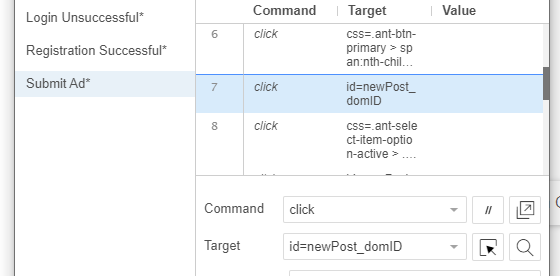
\includegraphics[scale=0.6]{slike/test10.PNG} %veličina slike u odnosu na originalnu datoteku i pozicija slike
				\centering
				\label{fig:test10}
			\end{figure}
			\begin{figure}[H]
				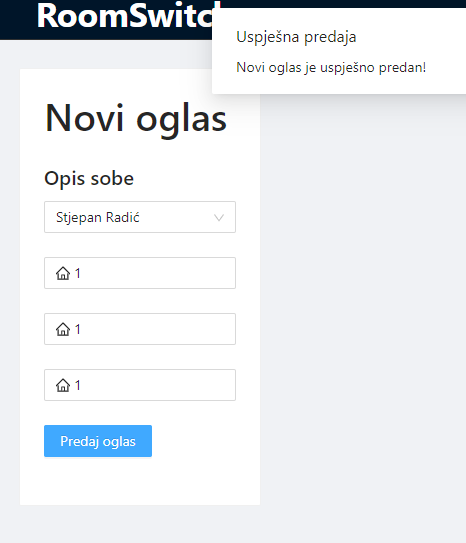
\includegraphics[scale=0.6]{slike/test10pom.PNG} %veličina slike u odnosu na originalnu datoteku i pozicija slike
				\centering
				\label{fig:test10pom}
			\end{figure}
			\begin{figure}[H]
				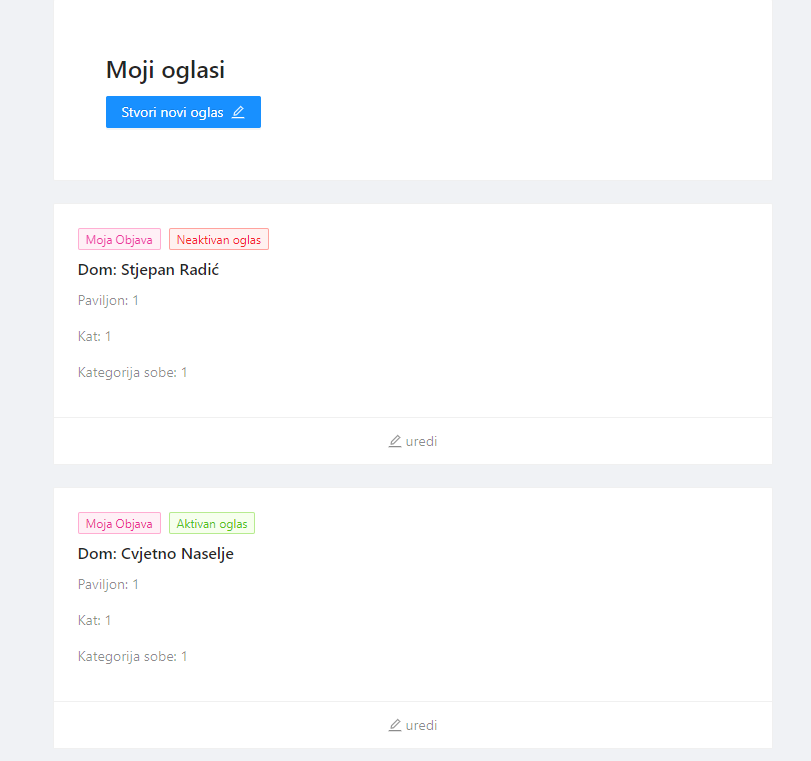
\includegraphics[scale=0.6]{slike/test10pompom.PNG} %veličina slike u odnosu na originalnu datoteku i pozicija slike
				\centering
				\label{fig:test10pom}
			\end{figure}
			
			\textbf{Ispitni slučaj 4: Ne prikazuj više ovaj oglas}	
			Testirano je označavanje oglasa da se više ne prikazuje te je očekivani rezultat početna stranica na kojoj nema označenog oglasa.
			
			\begin{figure}[H]
				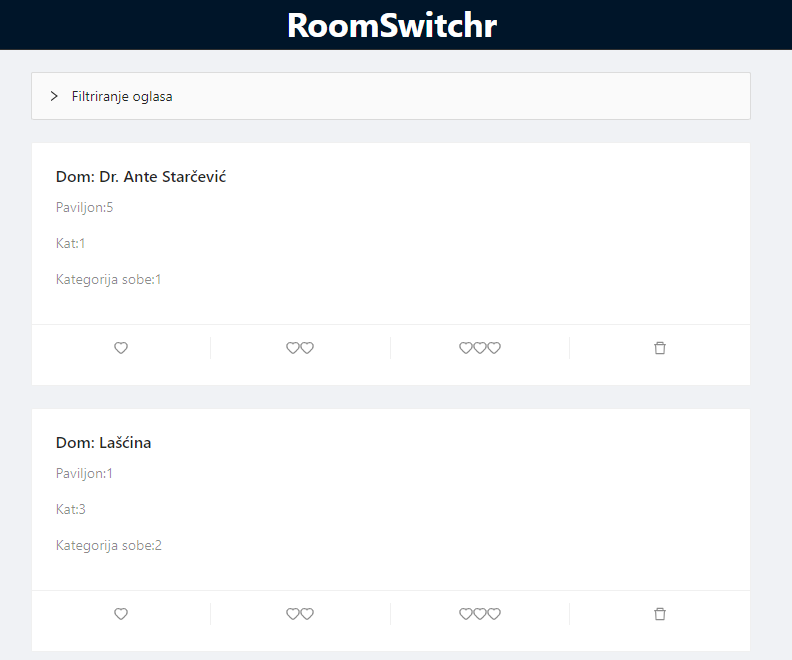
\includegraphics[scale=0.6]{slike/test11.PNG} %veličina slike u odnosu na originalnu datoteku i pozicija slike
				\centering
				\label{fig:test11}
			\end{figure}
			\begin{figure}[H]
				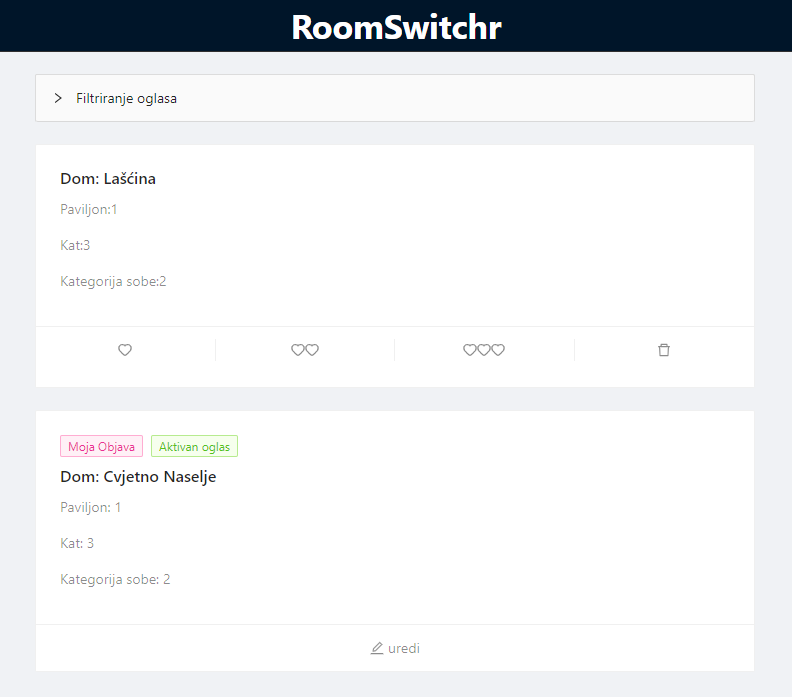
\includegraphics[scale=0.6]{slike/test11pom.PNG} %veličina slike u odnosu na originalnu datoteku i pozicija slike
				\centering
				\label{fig:test11pom}
			\end{figure}
			
			\eject 
		
		
		\section{Dijagram razmještaja}
			
			Dijagrami razmjestaja opisuju topologiju sklopovlja i programsku potporu koja se koristi u implementaciji sustava u njegovom radnom okruzenju. Na poslu žiteljskom
računalu se nalaze web poslužitelj i poslužitelj baze podataka. Klijenti koriste web preglednik kako bi pristupili web aplikaciji. Sustav je baziran na arhitekturi ”klijent – posluzitelj”, a komunikacija između računala korisnika (student ili djelatnik studentskog centra) i poslužitelja odvija se preko HTTP veze.
		
		\begin{figure}[H]
				\includegraphics[scale=0.5]{slike/dijag_razmještaja.PNG} %veličina slike u odnosu na originalnu datoteku i pozicija slike
				\centering
				\caption{Dijagram razmještaja}
				\label{fig:java}
			\end{figure}
			
			\eject
		
		\section{Upute za puštanje u pogon}

Potrebno je preuzeti PostgreSQL bazu podataka. Nakon toga potrebno je provesti standardnu instalaciju 
te se prijaviti s korisničkim imenom „postgres“ i lozinkom „bazepodataka“. 
Nakon instalacije, potrebno je pokrenuti pgAdmin i konfigurirati prvu konekciju na bazu. Potrebno je 
prijaviti se s istim korisničkim imenom i lozinkom kao i prilikom instalacije. U bazi podataka bi već 
trebala postojati tablica „postgres“. 
Server baze mora biti pokrenut. U daljnjim uputama opisan je način podizanja baze.
\vspace{3mm}

Kako bi se aplikacija pokrenula potrebno je instalirati podršku za bazu podataka, podršku za 
prevođenje i pokretnaje aplikacija napisanih u programskom jeziku Java te podršku za 
prevođenje i pokretnaje aplikacija napisanih u programskom jeziku JavaScript.
\vspace{3mm}

Prilikom instalacije podrške za bazu podataka potrebno je preuzeti aplikaciju pgAdmin s poveznice
\url{https://www.pgadmin.org/download/}. Nakon preuzimanja, potrebno je provesti standardnu instalaciju 
te se prijaviti s korisničkim imenom „postgres“ i lozinkom „bazepodataka“.
Nakon instalacije, potrebno je pokrenuti pgAdmin i konfigurirati prvu konekciju na bazu. Potrebno je 
prijaviti se s istim korisničkim imenom i lozinkom kao i prilikom instalacije. U bazi podataka bi već 
trebala postojati tablica „postgres“. Server baze tijekom korištenja aplikacije mora biti pokrenut.
Na računalu je također potrebno instalirati podršku za programski jezik Java (\url{http://jdk.java.net/15}).
Također kako bi se mogli pokretati programi napisani u JavaScriptu potrebno je instalirati Node.js 
(\url{https://nodejs.org/en/download}). 
\vspace{3mm}
Osim podrški za pokretanje programa, potrebno je instalirati i razvojnu okolinu. Najjednostavnije je instalirati
IDE Intelij jer se u njemu mogu pokretati programi napisani i u jeziku Java i u jeziku JavaScript.
Projekt se može preuzeti s poveznice \url{https://gitlab.com/mariakatic/piccologrupa}.
Nakon uspješne isntalacije svega od navedenog, konačno se može pokrenuti aplikacija. 
Potrebno je instalirati npm pakete pokretanjem naredbe npm install. Frontend se pokreće naredbom npm start, a 
backend pritiskom tipke Run u razvojnom okruženju.
Nakon pokretanja programa, aplikacija se može pregledati u pregledniku na poveznici http://localhost:3000.
\vspace{3mm}
Na gore opisan način pokreće se aplikacija neovisno o tome je li deployana. Ova aplikacija hostana je na 
cloud platofrmi Heroku te se također može pronaći na linku \url{https://switchr.herokuapp.com}.
			
			
			\eject 
	\chapter{Zaključak i budući rad}
		
		
		
Zadatak naše grupe bio je razvoj web aplikacije za olakšanu zamjenu soba u studentskim domovima. Aplikacija automatizira pronalazak mogućih kandidata za zamjenu te informiranje studentskog centra. Izrada projekta izvršena je kroz dva koraka.
Prvi korak uključivao je okupljanje tima, analiziranje zahtjeva zadatka, dogovor o raspodjeli posla i pisanje dokumentacije. Izrada obrazaca i dijagrama te detaljan opis rada aplikacije pomogli su pri ubrzanju razvoja u drugom koraku. Također je omogućeno razdvajanje posla na backend i frontend jer je njihova interakcija unaprijed određena. Što se tiče same aplikacije, izrađen je kostur na koji su se mogle brže i učinkovitije dodavati tražene funkcionalnosti.
Drugi korak bio je sama izrada aplikacije u obliku pisanja izvornog koda i dizajniranja korisničkog sučelja. U ovom koraku rađeno je i temeljito testiranje funkcionalnosti što je dovelo do brojnih inaćica rješenja tokom ispravljanja grešaka. Dokumentacija je u drugoj fazi nadopunjena i proširena po potrebi zbog novih ideja i unaprijed nepredviđenih slučajeva korištenja.
Moguće proširenje mogućnosti aplikacije je prijava zamjena dogovorenih izvan aplikacije radi lakše interakcije sa studentskim centrom, naprednije upravljanje oglasima i filtriranjem te poboljšanje sigurnosti podataka. Također je moguće izraditi i mobilnu aplikaciju kojom bi se povećala pristupačnost usluge koju projekt pruža.
Sudjelovanje na ovom projektu svim je članovima tima pružilo iskustvo u timskom radu na većem projektu. Shvatili smo potrebu za dobrom dokumentacijom i koordinacijom između članova pri svakom koraku razvoja. Iako završen projekt ima još mnogo prostora za poboljšanje zbog neiskustva sa ovakvom vrstom zadatka, zadovoljni smo onime što smo postigli.

		
		
		\eject 
	\chapter*{Popis literature}
		\addcontentsline{toc}{chapter}{Popis literature}
	 	
		
		
		\begin{enumerate}
			
			
			\item  Programsko inženjerstvo, FER ZEMRIS, \url{http://www.fer.hr/predmet/proinz}
			
			\item  I. Sommerville, "Software engineering", 8th ed, Addison Wesley, 2007.
			
			\item  ERDPlus, https://erdplus.com/
			
			\item Astah Community, http://astah.net/editions/uml-new
			
			\item  https://www.bu.edu/housing/assignments/changes/requests/room-change-requests-walkthrough/
			
		\end{enumerate}
		
		 
	\chapter*{Dodatak: Prikaz aktivnosti grupe}
		\addcontentsline{toc}{chapter}{Dodatak: Prikaz aktivnosti grupe}
		
		\section*{Dnevnik sastajanja}
		
		
		\begin{packed_enum}
			\item  sastanak
			
			\item[] \begin{packed_item}
				\item Datum: 29. rujna 2020.
				\item Prisustvovali: D.Ivezić, A.Trejić, B.Tolj, J.Ružić, D.Bokan, M.Katić
				\item Teme sastanka:
				\begin{packed_item}
					\item  odabran voditelj tima i ime tima
				\end{packed_item}
			\end{packed_item}
			
			\item  sastanak
			\item[] \begin{packed_item}
				\item Datum: 8. listopada 2020.
				\item Prisustvovali: D.Ivezić, A.Trejić, B.Tolj, J.Ružić, D.Bokan, M.Katić
				\item Teme sastanka:
				\begin{packed_item}
					\item  sastanak s asistenticom i demosom
					\item  analiza zadatka
				\end{packed_item}
			\end{packed_item}
			
			\item  sastanak
			\item[] \begin{packed_item}
				\item Datum: 12. listopada 2020.
				\item Prisustvovali: D.Ivezić, A.Trejić, B.Tolj, J.Ružić, D.Bokan, M.Katić
				\item Teme sastanka:
				\begin{packed_item}
					\item  dogovor oko alata i tehnologije
					\item  podjela rada
				\end{packed_item}
			\end{packed_item}
			
			\item  sastanak
			\item[] \begin{packed_item}
				\item Datum: 21. listopada 2020.
				\item Prisustvovali: D.Ivezić, A.Trejić, B.Tolj, J.Ružić, D.Bokan, M.Katić
				\item Teme sastanka:
				\begin{packed_item}
					\item  sastanak s asistenticom i demosom
					\item  analiza zadatka
					\item  nejasnoće u implementaciji generičkih funkcionalnosti
				\end{packed_item}
			\end{packed_item}
			
			\item  sastanak
			\item[] \begin{packed_item}
				\item Datum: 22. listopada 2020.
				\item Prisustvovali: D.Ivezić, A.Trejić, B.Tolj, J.Ružić, D.Bokan, M.Katić
				\item Teme sastanka:
				\begin{packed_item}
					\item  ispravljanje pogrešaka u implementaciji
				\end{packed_item}
			\end{packed_item}
			
			\item  sastanak
			\item[] \begin{packed_item}
				\item Datum: 5. studenog 2020.
				\item Prisustvovali: D.Ivezić, A.Trejić, B.Tolj, J.Ružić, D.Bokan, M.Katić
				\item Teme sastanka:
				\begin{packed_item}
					\item  sastanak s asistenticom i demosom
					\item  razrješavanje nejasnoća oko implementacije
				\end{packed_item}
			\end{packed_item}
			
			
			\item  sastanak
			\item[] \begin{packed_item}
				\item Datum: 10. studenog 2020.
				\item Prisustvovali: D.Ivezić, A.Trejić, B.Tolj, J.Ružić, D.Bokan, M.Katić
				\item Teme sastanka:
				\begin{packed_item}
					\item  sastanak s asistenticom
					\item  pregled dokumentacije
				\end{packed_item}
			\end{packed_item}
			
			
			\item  sastanak
			\item[] \begin{packed_item}
				\item Datum: 12. studenog 2020.
				\item Prisustvovali: D.Ivezić, A.Trejić, B.Tolj, J.Ružić, D.Bokan, M.Katić
				\item Teme sastanka:
				\begin{packed_item}
					\item  sastanak s asistenticom i demosom
					\item  demonstracija generičkih funkcionalnosti aplikacije
				\end{packed_item}
			\end{packed_item}
			
			\item  sastanak
			\item[] \begin{packed_item}
				\item Datum: 14. prosinca 2020.
				\item Prisustvovali: D.Ivezić, A.Trejić, B.Tolj, J.Ružić, D.Bokan, M.Katić
				\item Teme sastanka:
				\begin{packed_item}
					\item  podjela zadataka između članova
				\end{packed_item}
			\end{packed_item}
			
			\item  sastanak
			\item[] \begin{packed_item}
				\item Datum: 22. prosinca 2020.
				\item Prisustvovali: D.Ivezić, A.Trejić, B.Tolj, J.Ružić, D.Bokan, M.Katić
				\item Teme sastanka:
				\begin{packed_item}
					\item  pregled trenutno napravljenog
					\item  razjašnjenje nejasnoća
				\end{packed_item}
			\end{packed_item}
			
			\item  sastanak
			\item[] \begin{packed_item}
				\item Datum: 4. siječnja 2021.
				\item Prisustvovali: D.Ivezić, A.Trejić, B.Tolj, J.Ružić, D.Bokan, M.Katić
				\item Teme sastanka:
				\begin{packed_item}
					\item  razjašnjenje nejasnoća
					\item  analiza traženih zadataka
					\item  podjela ostatka posla i dokumentacije
				\end{packed_item}
			\end{packed_item}
			
			\item  sastanak
			\item[] \begin{packed_item}
				\item Datum: 7. siječnja 2021.
				\item Prisustvovali: D.Ivezić, A.Trejić, B.Tolj, J.Ružić, D.Bokan, M.Katić
				\item Teme sastanka:
				\begin{packed_item}
					\item  sastanak s asistenticom i demosom
					\item  demonstracija alfa verzije
				\end{packed_item}
			\end{packed_item}
			
			\item  sastanak
			\item[] \begin{packed_item}
				\item Datum: 8. siječnja 2021.
				\item Prisustvovali: D.Ivezić, A.Trejić, B.Tolj, J.Ružić, D.Bokan, M.Katić
				\item Teme sastanka:
				\begin{packed_item}
					\item  pregled trenutno napravljenog
					\item  popravljanje grešaka u kodu
				\end{packed_item}
			\end{packed_item}
			
			\item  sastanak
			\item[] \begin{packed_item}
				\item Datum: 13. siječnja 2021.
				\item Prisustvovali: D.Ivezić, A.Trejić, B.Tolj, J.Ružić, D.Bokan, M.Katić
				\item Teme sastanka:
				\begin{packed_item}
					\item  spajanje backenda i frontenda
				\end{packed_item}
			\end{packed_item}
			
			%
			
		\end{packed_enum}
		
		\eject
		\section*{Tablica aktivnosti}
		
					
						
			
			\begin{longtabu} to \textwidth {|X[7, l]|X[1, c]|X[1, c]|X[1, c]|X[1, c]|X[1, c]|X[1, c]|X[1, c]|}
								
				\cline{2-8} \multicolumn{1}{c|}{\textbf{}} &     \multicolumn{1}{c|}{\rotatebox{90}{\textbf{Maria Katić }}} & \multicolumn{1}{c|}{\rotatebox{90}{\textbf{Ajdin Trejić }}} &	\multicolumn{1}{c|}{\rotatebox{90}{\textbf{Dora Ivezić }}} &	\multicolumn{1}{c|}{\rotatebox{90}{\textbf{Daniel Bokan }}} &
				\multicolumn{1}{c|}{\rotatebox{90}{\textbf{Josipa Ružić }}} &
				\multicolumn{1}{c|}{\rotatebox{90}{\textbf{Bruno Tolj }}} &	\multicolumn{1}{c|}{\rotatebox{90}{\textbf{x }}} \\ \hline 
				\endfirsthead
				

				
				
				\endfoot
							
				 
				\endlastfoot
				
				Upravljanje projektom 		&2  &  &  &  &  &  & \\ \hline
				Opis projektnog zadatka 	&2  &  &  &  &  &  & \\ \hline
				
				Funkcionalni zahtjevi       &  &  &  &  &1  &  &  \\ \hline
				Opis pojedinih obrazaca 	&  &  &  &  &8  &  &  \\ \hline
				Dijagram obrazaca 			&  &  &  &  &1  &  &  \\ \hline
				Sekvencijski dijagrami 		&  &  &  &  &2  &  &  \\ \hline
				Opis ostalih zahtjeva 		&  &  &  &  &1  &  &  \\ \hline

				Arhitektura i dizajn sustava	 &  &  &3  &  &  &  &  \\ \hline
				Baza podataka				&  &  &4  &  &  &  &   \\ \hline
				Dijagram razreda 			&  &  &4  &  &  &  &   \\ \hline
				Dijagram stanja				&  &  &  &  &2  &  &  \\ \hline
				Dijagram aktivnosti 		&  &  &  &  &2 &  &  \\ \hline
				Dijagram komponenti			&1  &  &  &  &  &  &  \\ \hline
				Korištene tehnologije i alati 		&  &  &  &  &  &1  &  \\ \hline
				Ispitivanje programskog rješenja 	&1  &  &  &2  &  &  &  \\ \hline
				Dijagram razmještaja			&  &  &  &  &1  &  &  \\ \hline
				Upute za puštanje u pogon 		&  &1  &  &  &  &  &  \\ \hline 
				Dnevnik sastajanja 			&1  &  &  &  &  &  &  \\ \hline
				Zaključak i budući rad 		&  &  &  &  &  &1  &  \\  \hline
				Popis literature 			&1  &  &  &  &  &  &  \\  \hline
				&  &  &  &  &  &  &  \\ \hline \hline
				\textit{Dodatne stavke kako ste podijelili izradu aplikacije} 			&  &  &  &  &  &  &  \\ \hline
				\textit{npr. izrada početne stranice} 				&  &40  &40  &  &  &  &  \\ \hline 
				\textit{izrada baze podataka} 		 			&1  &6  &  &  &  &  & \\ \hline 
				\textit{spajanje s bazom podataka} 							&  &  &  &4  &  &  &  \\ \hline
				\textit{back end} 							&40  &3  &  &40  &10  &40  &  \\  \hline
				
				
			\end{longtabu}
			
			\section*{Dijagrami pregleda promjena}
			
			%unos slike
		\begin{figure}[H]
			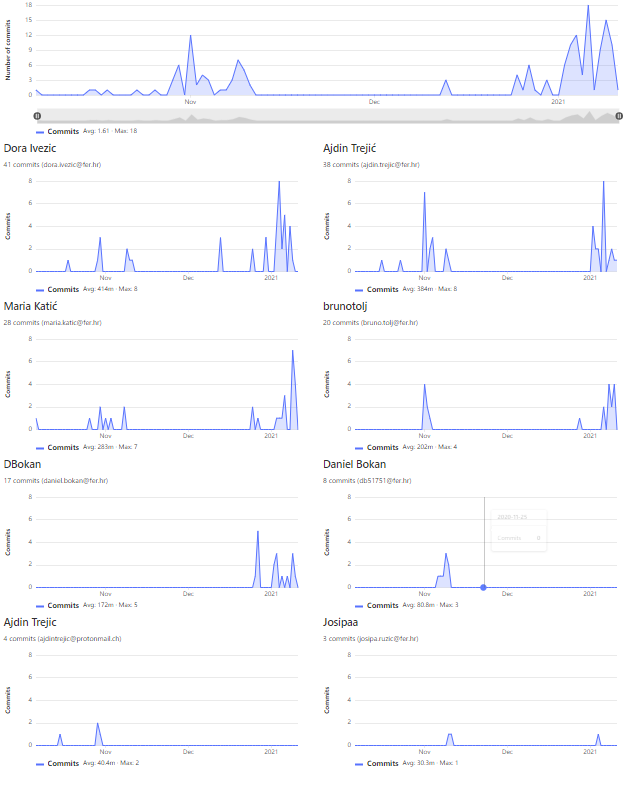
\includegraphics[scale=0.9]{slike/aktivnost.PNG} %veličina slike u odnosu na originalnu datoteku i pozicija slike
			\centering
			\caption{Prikaz aktivnosti na repozitoriju}
			\label{fig:promjene}
		\end{figure}
					
					
		\eject
		
	
	
	
	\begingroup
	\renewcommand*\listfigurename{Indeks slika i dijagrama}
	%\renewcommand*\listtablename{Indeks tablica}
	%\let\clearpage\relax
	\listoffigures
	%\vspace{10mm}
	%\listoftables
	\endgroup
	\addcontentsline{toc}{chapter}{Indeks slika i dijagrama}


	
	\eject 



\end{document} %naredbe i tekst nakon ove naredbe ne ulaze u izgrađen dokument 


